\documentclass[11pt]{article}
%\usepackage{CJK,CJKspace}
\usepackage{hyperref}
\usepackage{url}
\usepackage{amsthm,enumitem}
\usepackage{graphicx}
\usepackage{algorithmic}
\usepackage{geometry}
\usepackage{setspace}
\usepackage{indentfirst}
\usepackage{epsfig,tabularx,amssymb,amsmath,subfigure,multirow}
%\usepackage[margin=0.5in]{geometry}
%\input myfonts
\newtheorem{lemma}{Lemma}

\newtheorem*{claim}{Claim}
\renewcommand{\baselinestretch}{1.5}
\newcommand{\nop}[1]{}
\begin{document}

\newgeometry{left=1in,right=1in,top=1in,bottom=1in}
\centerline{\bf \LARGE Visualization of MovieLens Rating}
\bigskip
\centerline{\bf \LARGE Process Book}
\bigskip
\bigskip
\centerline{\bf \Large Zhao Chang u0931132@utah.edu u0931132}
\centerline{\bf \Large Junwei Shi u0943296@utah.edu u0943296}
\centerline{\bf \Large Tengda Shi tengda.shi@utah.edu u1015168}
\bigskip
\centerline{\bf \Large Project Repository: \url{https://github.com/VaultB0Y/dataviscourse-pr-visualization}}

\section{Overview and Motivation}

The objective of our project is to perform an interactive visualization analysis on the relationship between different kinds of movies and people who give ratings on the movies. Our project deals with a really interesting problem. Note that thousands of movies are released over the world each year. We can easily find the corresponding information in some online web sites (eg. IMDB\footnote{\url{http://www.imdb.com/}}). However, in fact, we are only interested in a small part of them. We have no time to scan all the introductions to these movies. Thus, we hope we can perform an interactive visualization analysis and tell people what movies they may like to see based on people's attribute information. The attribute information regarding different people can also be added into existing recommendation systems and improve the accuracy of recommendation.

\section{Related Work}

Existing works regarding recommendation systems inspire us to finish such a project. There are three major approaches used in prior works. The first one is collaborative filtering. It has been used in a lot of highly cited papers \cite{WWW2001,IEEE2003}. It does not rely on profile information of users and items. Also, it does not need any knowledge engineering effort. However, it requires some form of rating feedback. Also, it cannot solve cold start for new users and new items \cite{IJCAI2013}. The second one is content-based recommendation. It has already been used in some early works regarding recommendation algorithms \cite{AAAI1998,DL2000}. It only makes comparisons between items possible and does not require any community information. However, it needs some necessary content descriptions. Also, it cannot solve cold start for new users. The third one is knowledge-based recommendation. It is also used in a few research works \cite{ELIS2000,WWW2008}. It makes deterministic recommendations and ensures the quality of recommended items. Also, it can solve the cold start problem. However, it only works for static recommendations well and does not react to short-term trends. Recently, there are also some new approaches proposed by researchers. For example, some works improve traditional recommendation systems by adding social network analysis \cite{WWW20082,UCS2011}. Some works extract entities in users' tweets or weibos and add such information into existing frameworks for achieving advanced recommendation systems \cite{RS2009,IR2011}.

However, all these works focus on how to recommend products for users accurately. These recommendation algorithms are usually performed based on some complicated mathematical deductions. However, it seems difficult for such algorithms to explain how they can generate reasonable results \emph{in an intuitive way}. Therefore, we need to utilize the visualization tools. We perform an interactive visualization analysis and tell people what movies they may like to see based on people��s attribute information.

The visualization in this web site\footnote{\url{http://benfry.com/isometricblocks/}} inspires us to design Figure \ref{fig:fig12}. Figure \ref{fig:fig12} can easily reveal the dependencies of users with different attributes and different kinds of movies.

\section{Questions}

The primary questions we are trying to answer with our visualization are:
\begin{itemize}
\item Tell people which movie they may like to see. If you plan to watch a movie but you are not sure if you will like this movie, then you can see the ratings of people who are in your ages through our visualization and decide whether to go to see the movie.
\item For people in different ages, check what their favorite movies are and the ratings of each certain movie. The basic function of our visualization is to provide the services for users to search the information they want to check about the movies.
\item Help the movie makers to investigate who like their movies best. Our visualization will also benefit the movie makers and help them to make movies that more people like to watch.
\end{itemize}

What we would like to learn is if any trends or patterns exist in our data set. In particular, the things we would like to accomplish include:
\begin{itemize}
\item Show all the ratings of each movie, including the information of people who generate these ratings.
\item Show different ratings of different movies generated by each person. People can search the information according to the audience's gender, occupation, postal zone and so on.
\item Movies can be searched by category, theme, year and so on.
\end{itemize}

How do these questions evolve over the course of the project?

\begin{itemize}
\item In our proposal, we mainly focus on the influence of the attribute "Age". As the project goes, we realize that "Location" and "Gender" can also have an influence on people's choices. For example, males usually give higher ratings for action movies, crime movies and thrillers than females, while females usually give higher ratings for children's movies, animations and comedies.
\end{itemize}

What new questions do you consider in the course of your analysis?
\begin{itemize}
\item As the project goes, we pay more attention to trying all kinds of data analyses. For example, we may answer the questions "What is the average rating for each genre of movies?", "Are old movies more highly-rated than new movies?", and "What kinds of movies do people in California like to see?", "How about the case in the whole America?". These interesting questions have not been mentioned in our proposal. However, over the course of the project, we discuss with each other for several times and gradually make our visualization work solid.
\end{itemize}

\section{Data}

We use MovieLens 1M Data Set\footnote{\url{http://datahub.io/dataset/movielens}}. This data set contains 1,000,209 ratings applied to 3,952 movies by 6,040 users of the online movie recommender service MovieLens. All ratings are contained in the file ``ratings.dat'' and are in the following format: UserID::MovieID::Rating::Timestamp. Ratings are made on a 5-star scale. Each user has at least 20 ratings. User information is in the file ``users.dat'' and is in the following format: UserID::Gender::Age::Occupation::Zip-code. Movie information is in the file ``movies.dat'' and is in the following format: MovieID::Title::Genres. By performing visualization analysis on the data set, we can answer some interesting questions, such as ``what kinds of movies are liked by people with some specific attributes''.

We pre-process the data set by clustering the data according to different kinds of movies and different attributes of people. After generating such aggregation information, we perform interactive visualization analysis on the transformed data set.

\section{Exploratory Data Analysis}

What visualizations do you use to initially look at your data?

\begin{itemize}
\item In our milestone, we use static bar charts, pie charts, tree maps, line charts and box plots to look at our data.
\end{itemize}

What insights do you gain?

\begin{itemize}
\item Different kinds of movies gain different numbers of ratings. Although comedies, dramas and action movies do not have higher average ratings, they gain much more ratings from all kinds of people.
\item Few people give ratings for documentaries and film noirs. However, these two kinds of movies gain the top two average ratings. It seems that only a few people pay attention to them and give them high ratings. For the majority of people, they even do not realize the existence of these movies.
\item Some information (eg. geo-location information) cannot be represented in such a simple way. Also, only using static visualization design has difficulty in showing people more detailed information in the data set.
\end{itemize}

How do these insights inform your design?

\begin{itemize}
\item There are some really interesting patterns that we need to find in our data set.
\item We may need to introduce a map to represent the geo-location information in the data set.
\item We may need to add more interactive data visualization designs in our project.
\end{itemize}

\section{Design Evolution}

\subsection{Our Design in Proposal}

In our design, we divide the whole framework into five parts:

\begin{itemize}
\item[1)] Present the rating information given a specific user.
\item[2)] Present the rating information given a specific movie.
\item[3)] Process the statistic given a specific user group using filtering.
\item[4)] Process the statistic given a specific movie group using filtering.
\item[5)] Find the dependencies of users with different attributes and different kinds of movies.
\end{itemize}

\subsubsection{Part 1 Design}
We can search the rating information given a specific user. Also we could filter out some types
of movies we do not need, such as released year and genres (as shown in Figure \ref{fig:fig1}). After that, we can present the
information grouped by genre, or just a scatter plot along the year x-axis. (see Figure \ref{fig:fig2} and \ref{fig:fig3}). Also
we can rank the movies as shown in Figure \ref{fig:fig11}.

\subsubsection{Part 2 Design}
We can search the rating information given a specific movie. We could present some interesting
statistics, such as number of ratings or scores, categorized by ages. (Figure \ref{fig:fig5} and \ref{fig:fig6}), or categorized
by some interesting features such as locations. Please note that Figure \ref{fig:fig6} is a distribution figure,
and we use different colors to denote the distribution percentage.

\subsubsection{Part 3 Design}
First we need to filter out the users we want, by selecting some features as in Figure \ref{fig:fig7}. Then we
show the statistics as Figure \ref{fig:fig5} and \ref{fig:fig6}.

\subsubsection{Part 4 Design}
We can filter out the movies by selecting features as shown in Figure \ref{fig:fig4}. We can show the statistics as shown in
Figure \ref{fig:fig9} and Figure \ref{fig:fig10}.

\subsubsection{Part 5 Design}
After some preprocessing of the data, such as clustering or collaborative filtering, we can show
the dependencies of different groups of users and the movies. The groups are based on the features
we have selected.

\begin{figure}[h]
\centering{
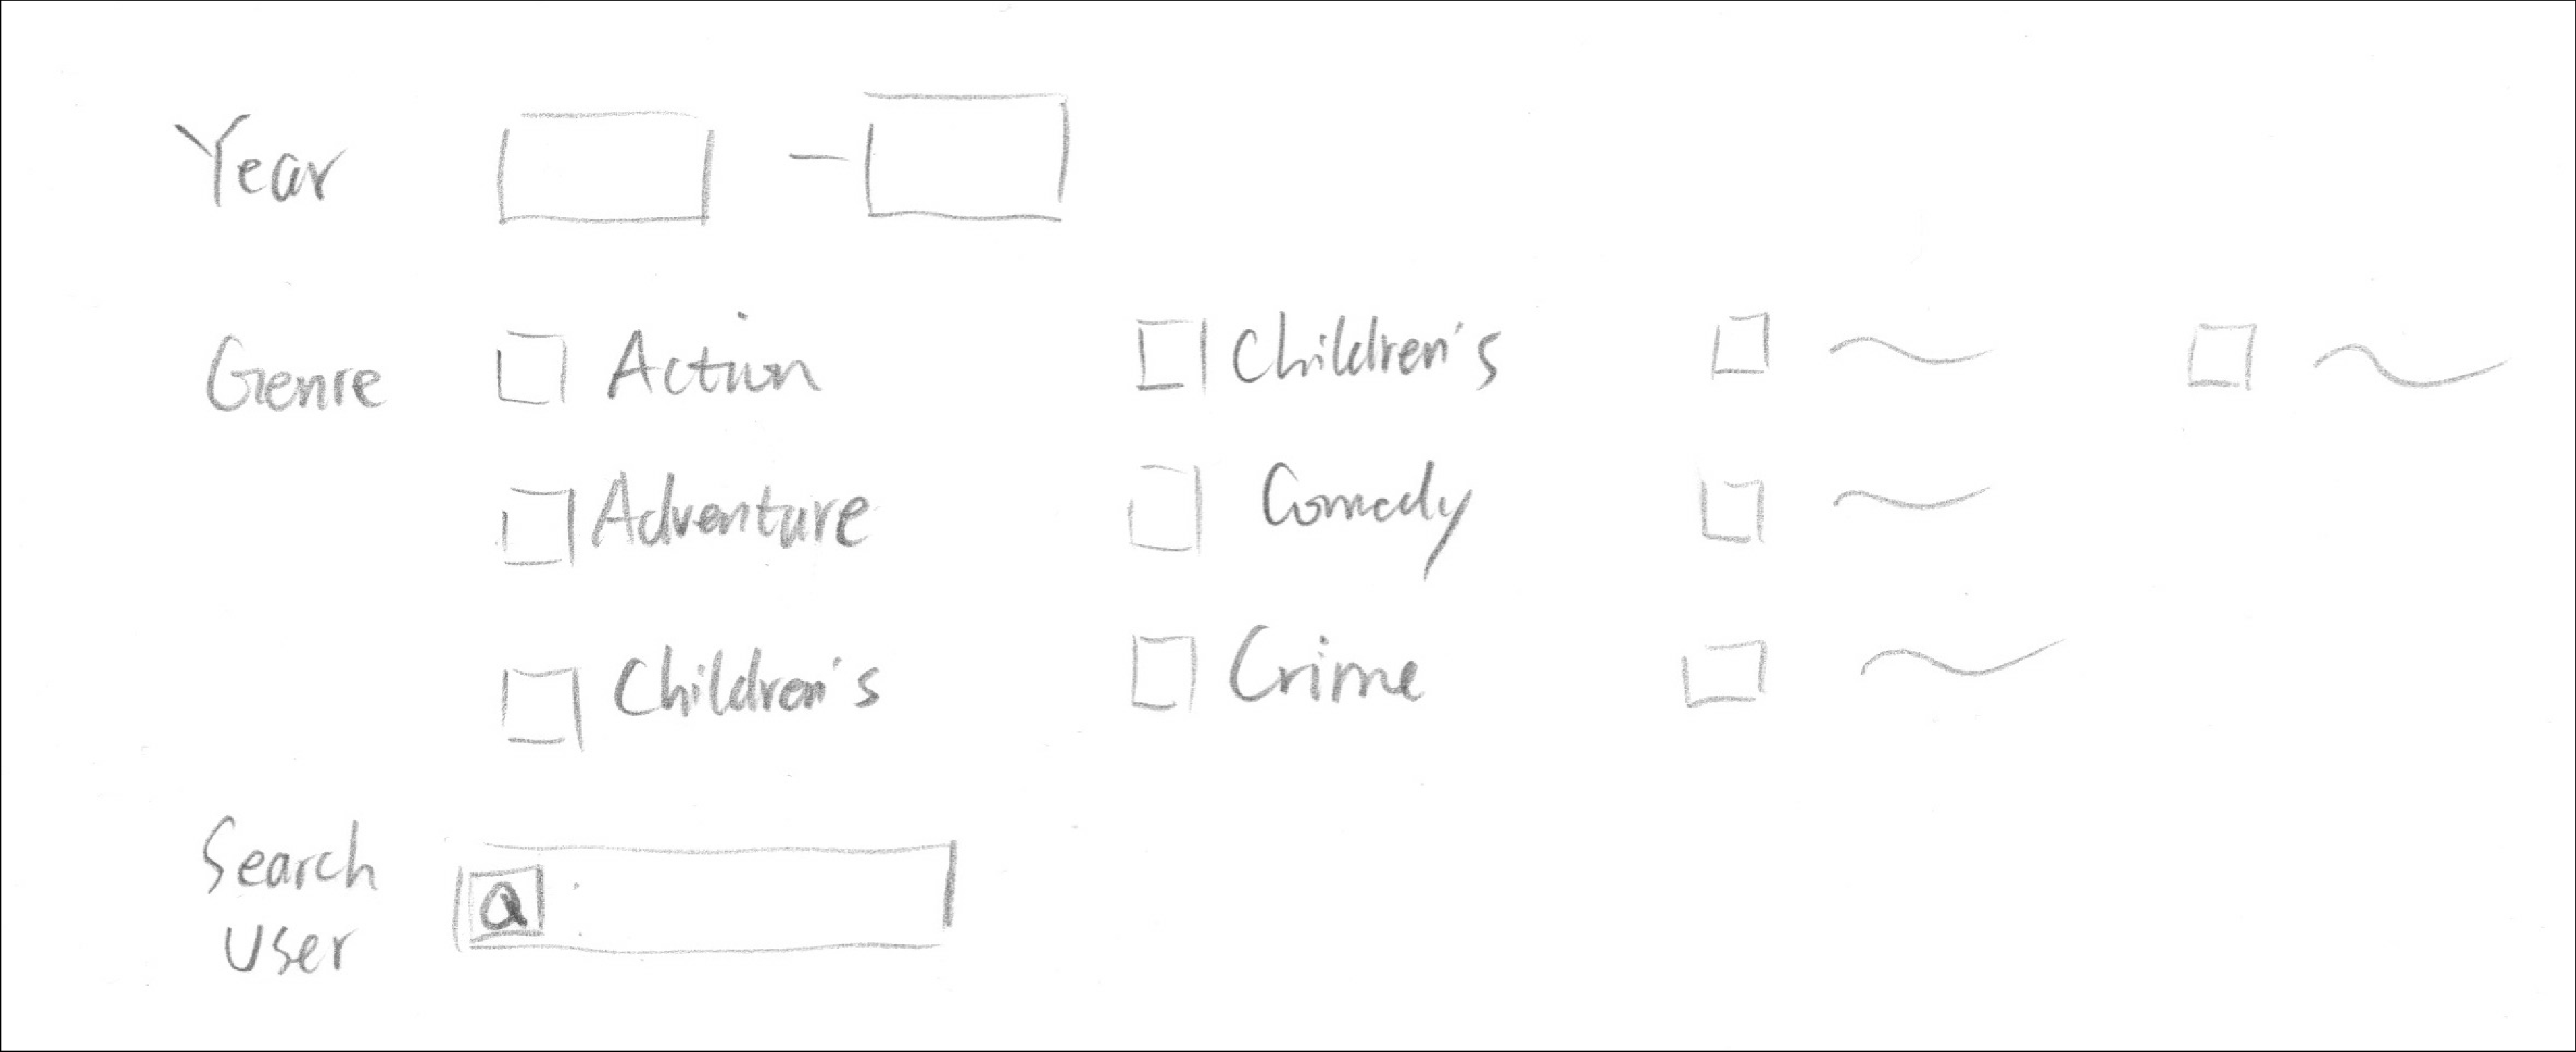
\includegraphics[width=.7\linewidth]{1.pdf}
}
\caption{Search for user and filter the movie information}
\label{fig:fig1}
\end{figure}

\begin{figure}[h]
\centering{
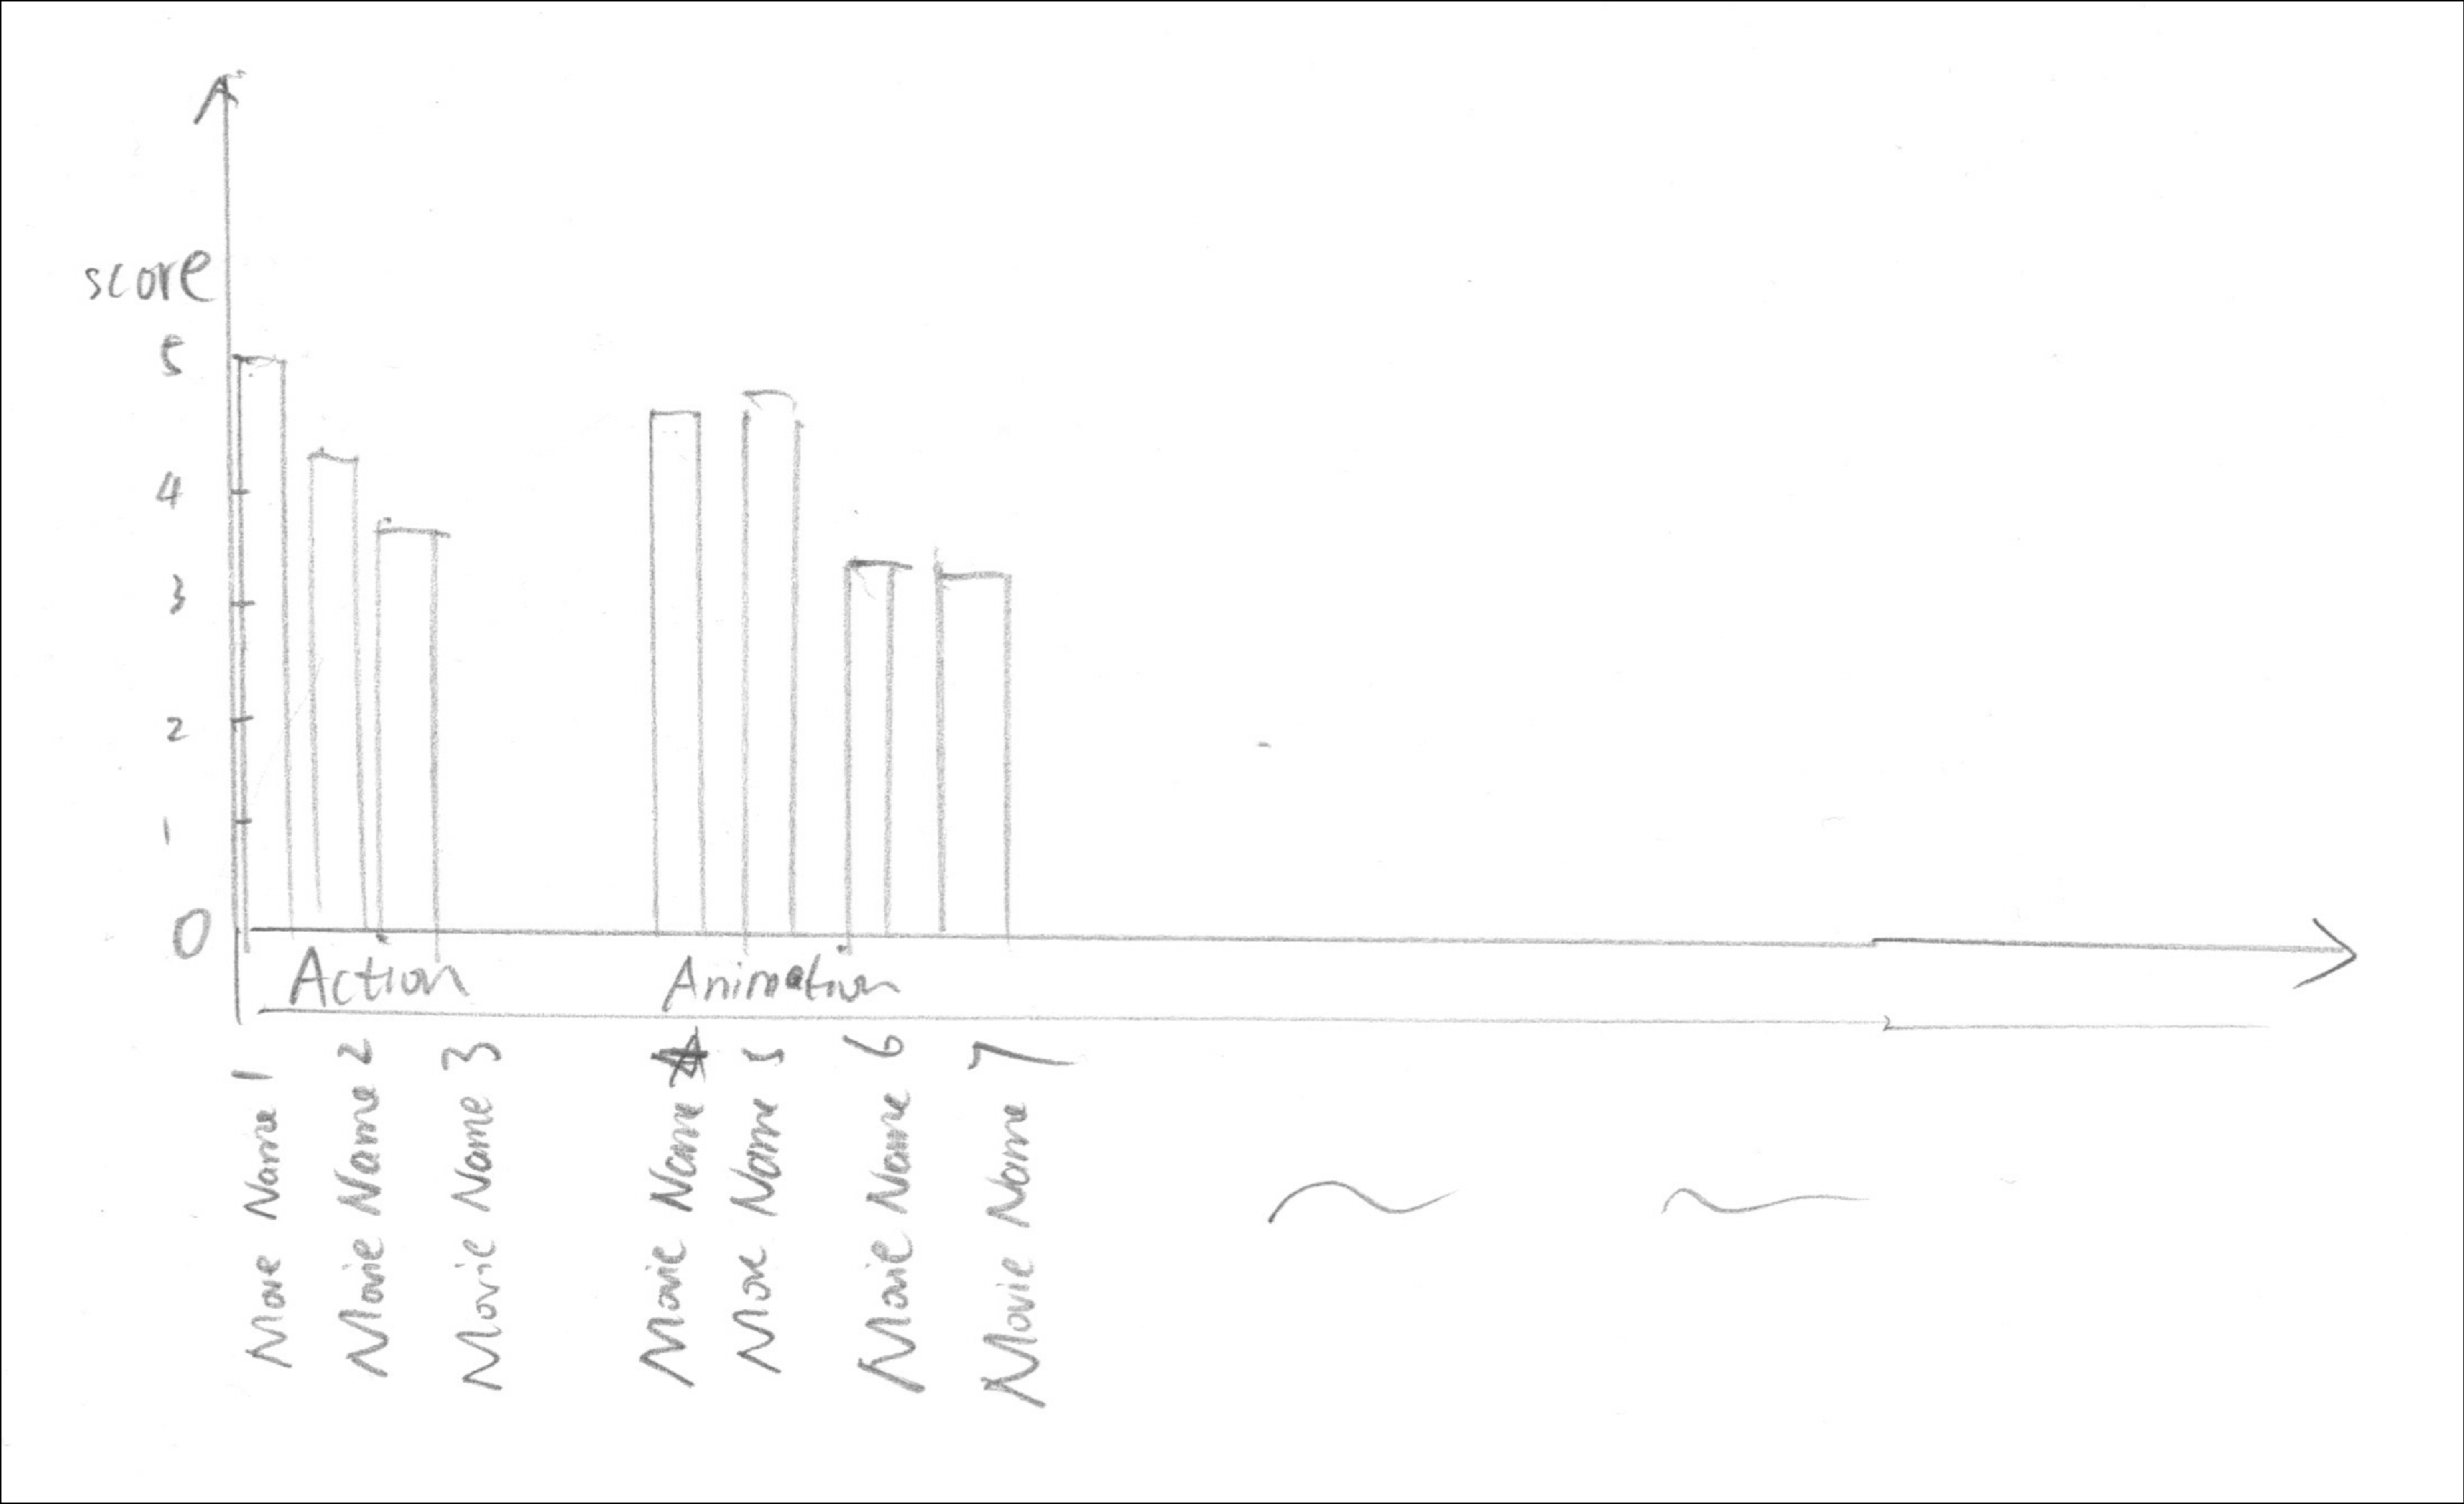
\includegraphics[width=.7\linewidth]{2.pdf}
}
\caption{Histogram of ratings grouped by genre}
\label{fig:fig2}
\end{figure}

\begin{figure}[h]
\centering{
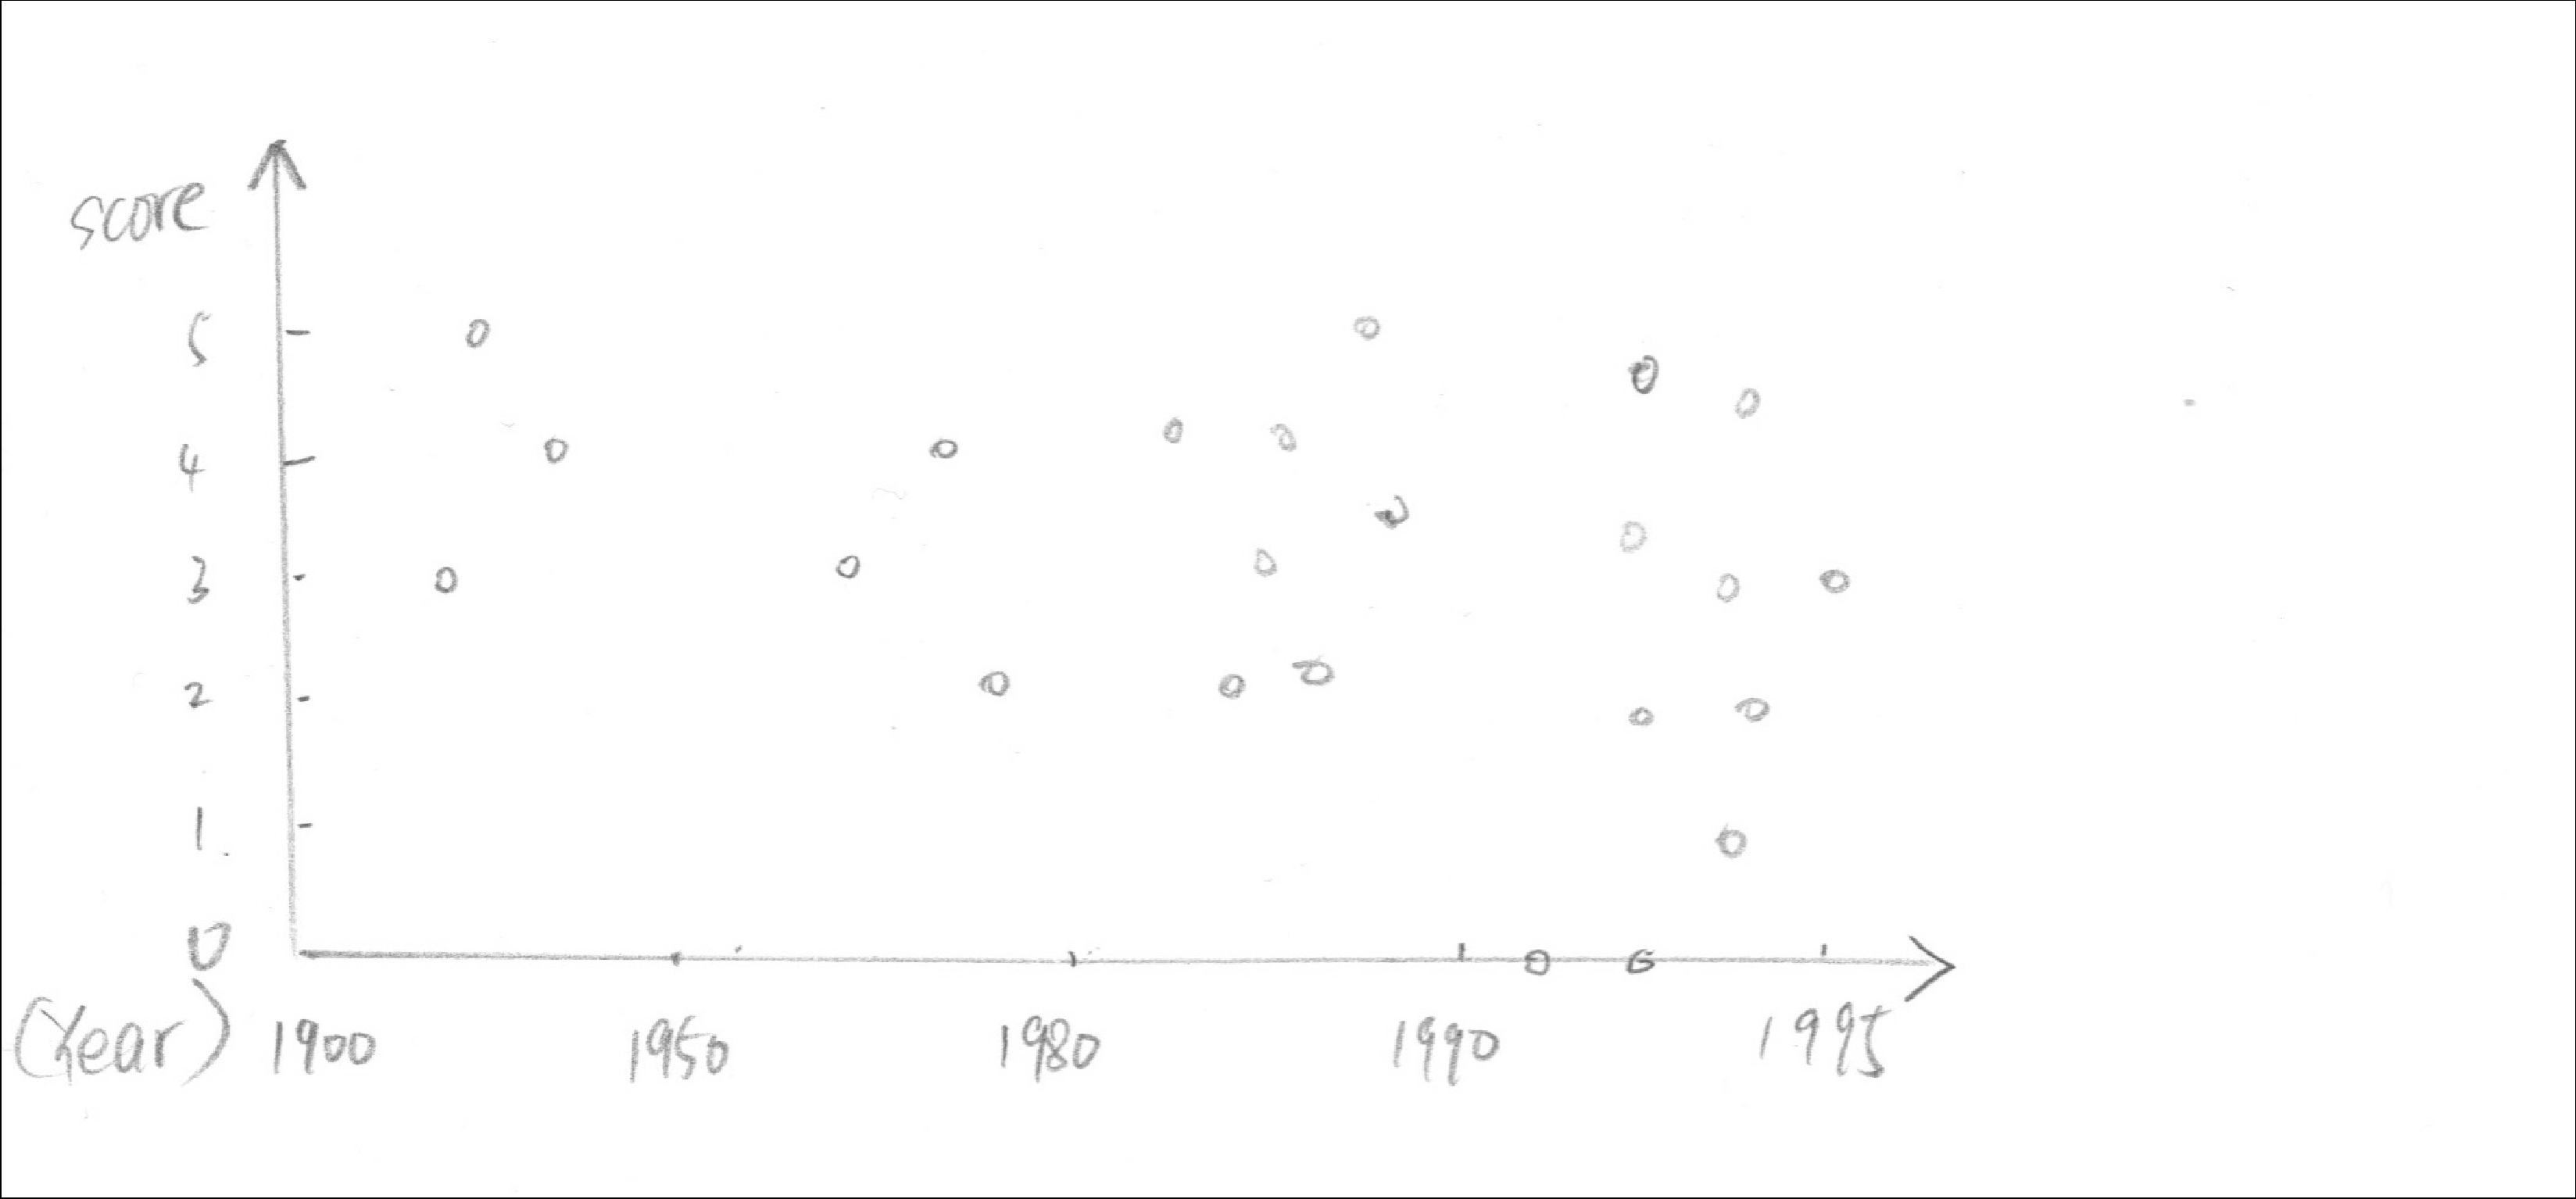
\includegraphics[width=.7\linewidth]{3.pdf}
}
\caption{Scatter plot of ratings}
\label{fig:fig3}
\end{figure}

\begin{figure}[h]
\centering{
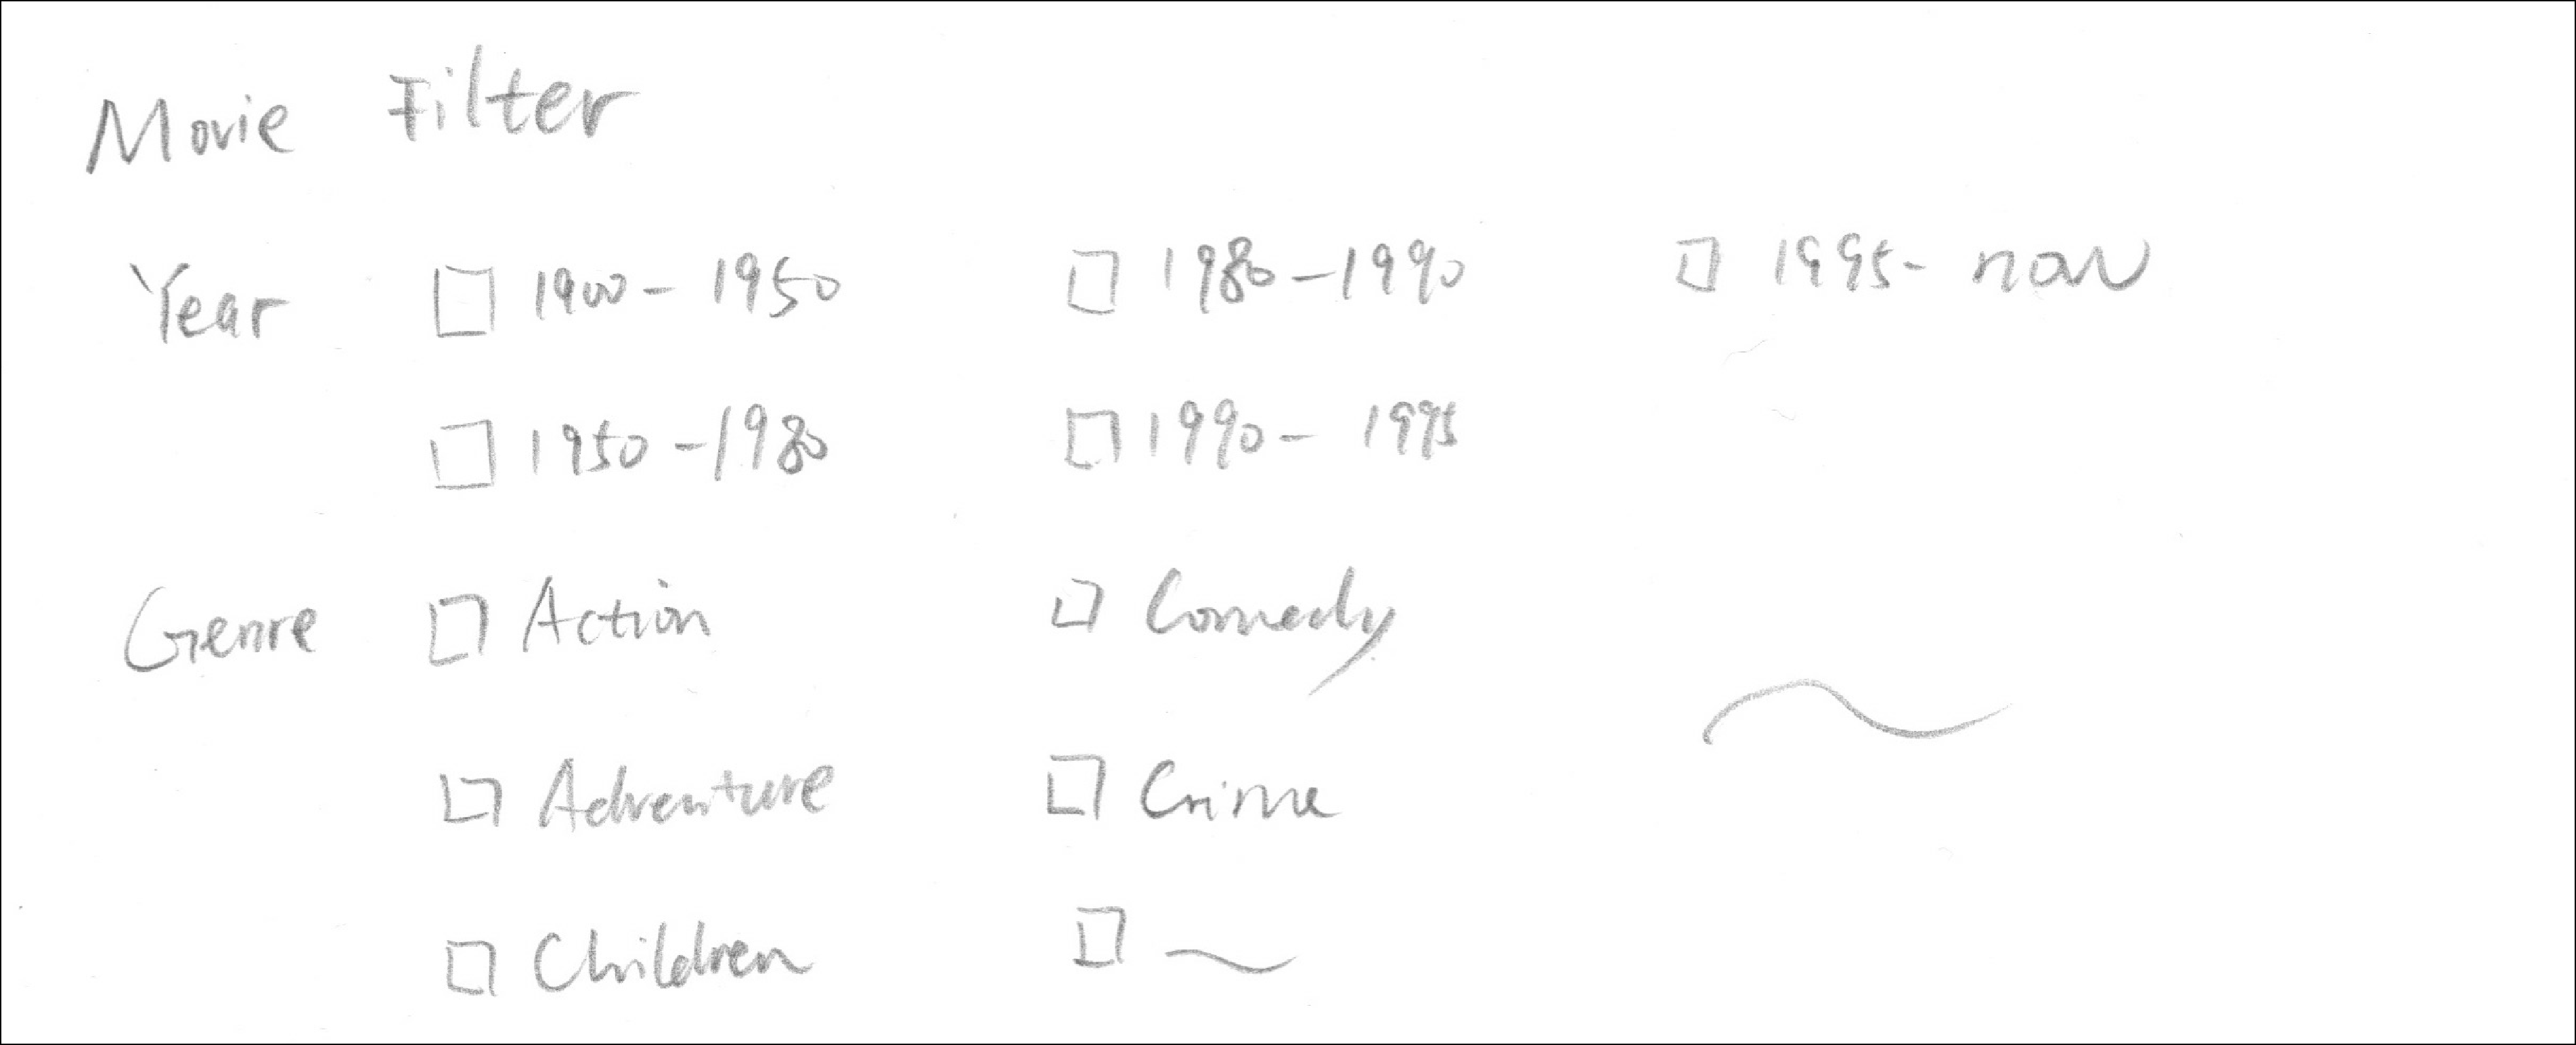
\includegraphics[width=.7\linewidth]{4.pdf}
}
\caption{Filter of movie information}
\label{fig:fig4}
\end{figure}

\begin{figure}[h]
\centering{
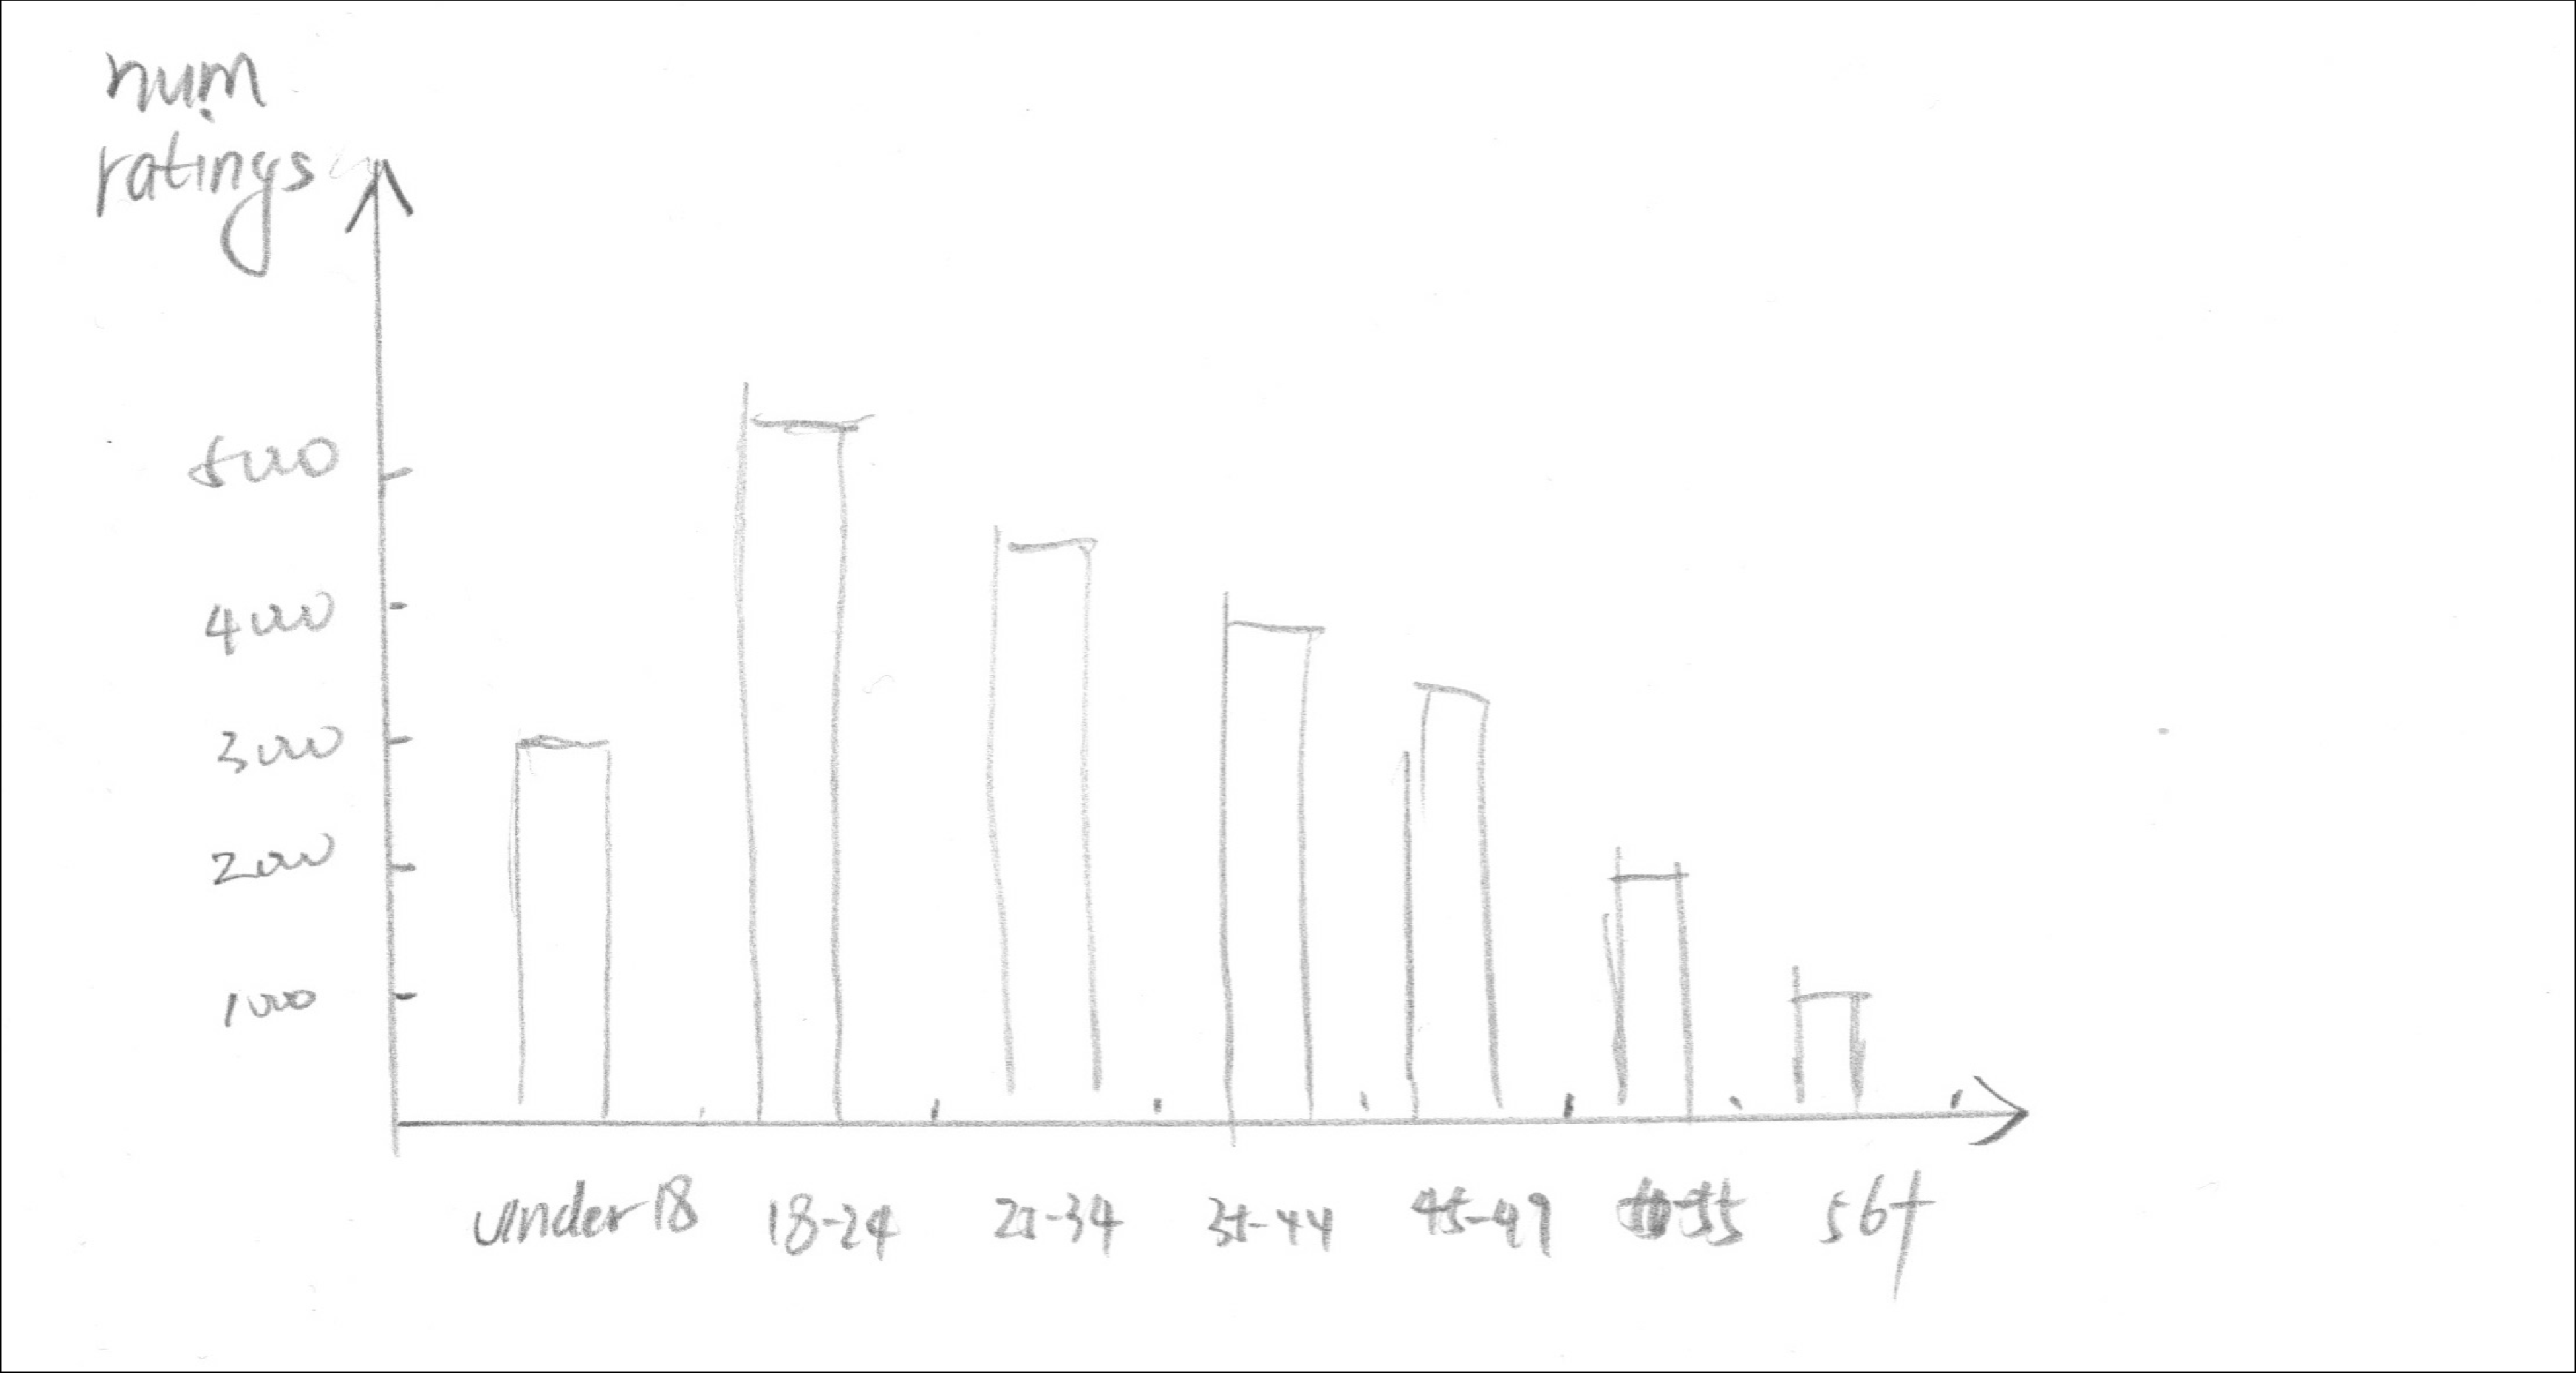
\includegraphics[width=.7\linewidth]{5.pdf}
}
\caption{Number of ratings grouped by ages}
\label{fig:fig5}
\end{figure}

\begin{figure}[h]
\centering{
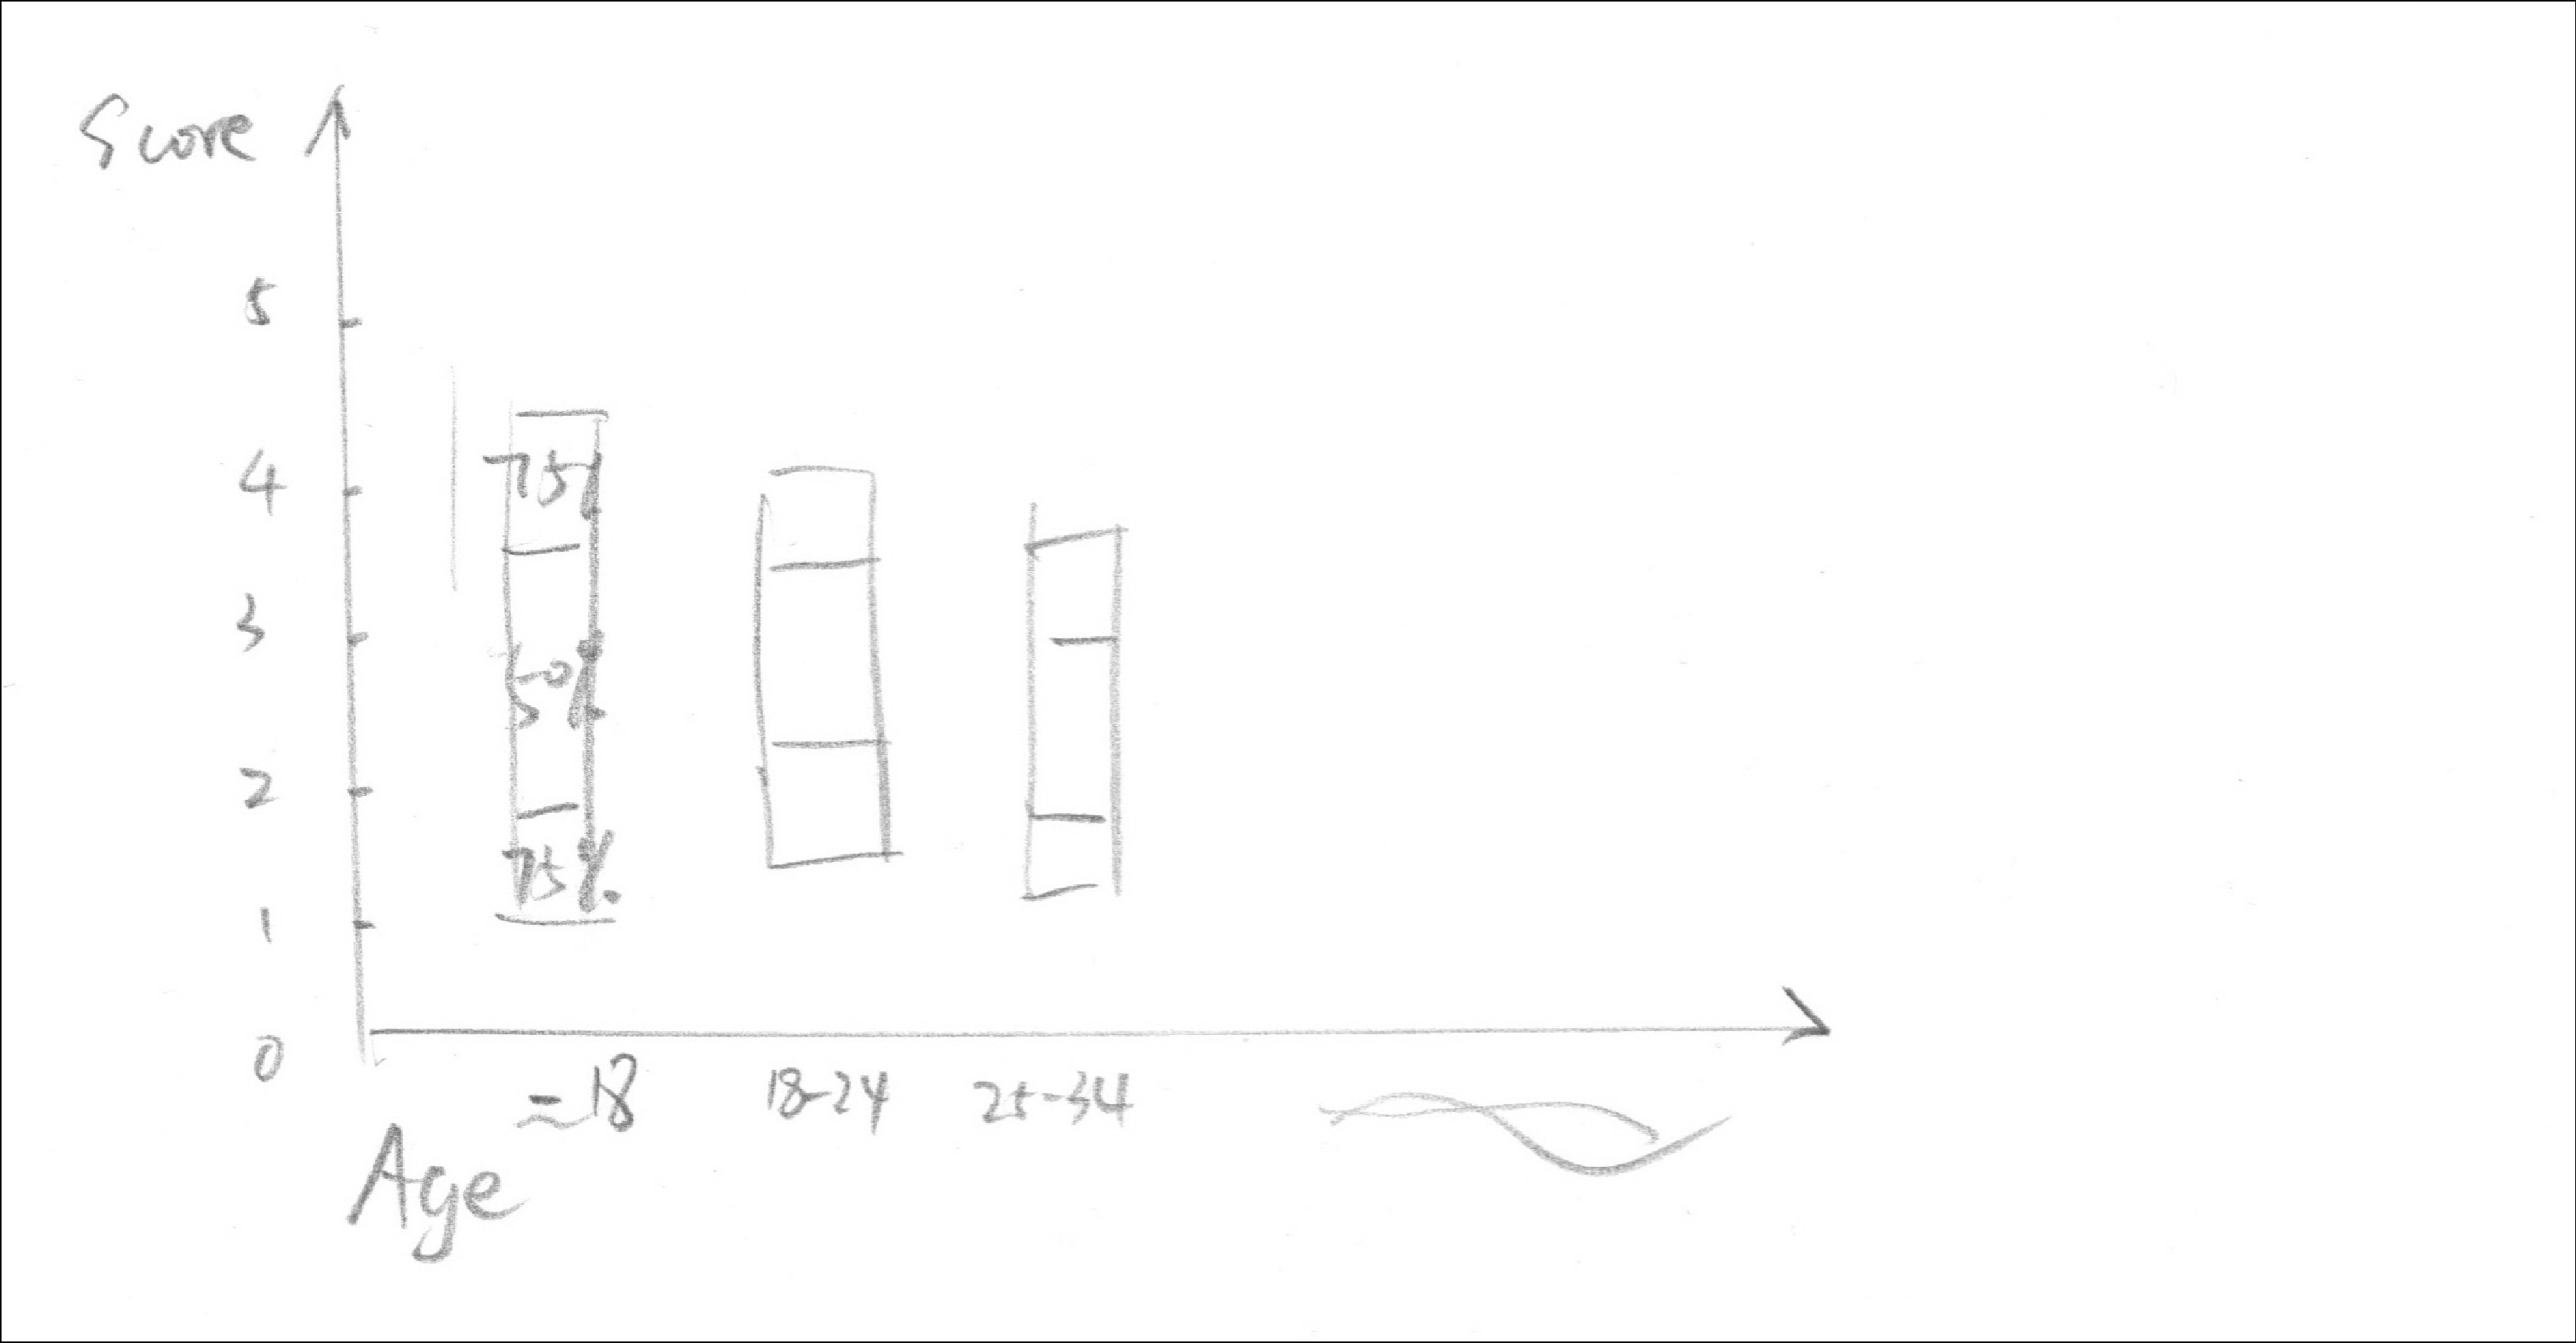
\includegraphics[width=.7\linewidth]{6.pdf}
}
\caption{Distributions of ratings grouped by ages}
\label{fig:fig6}
\end{figure}

\begin{figure}[h]
\centering{
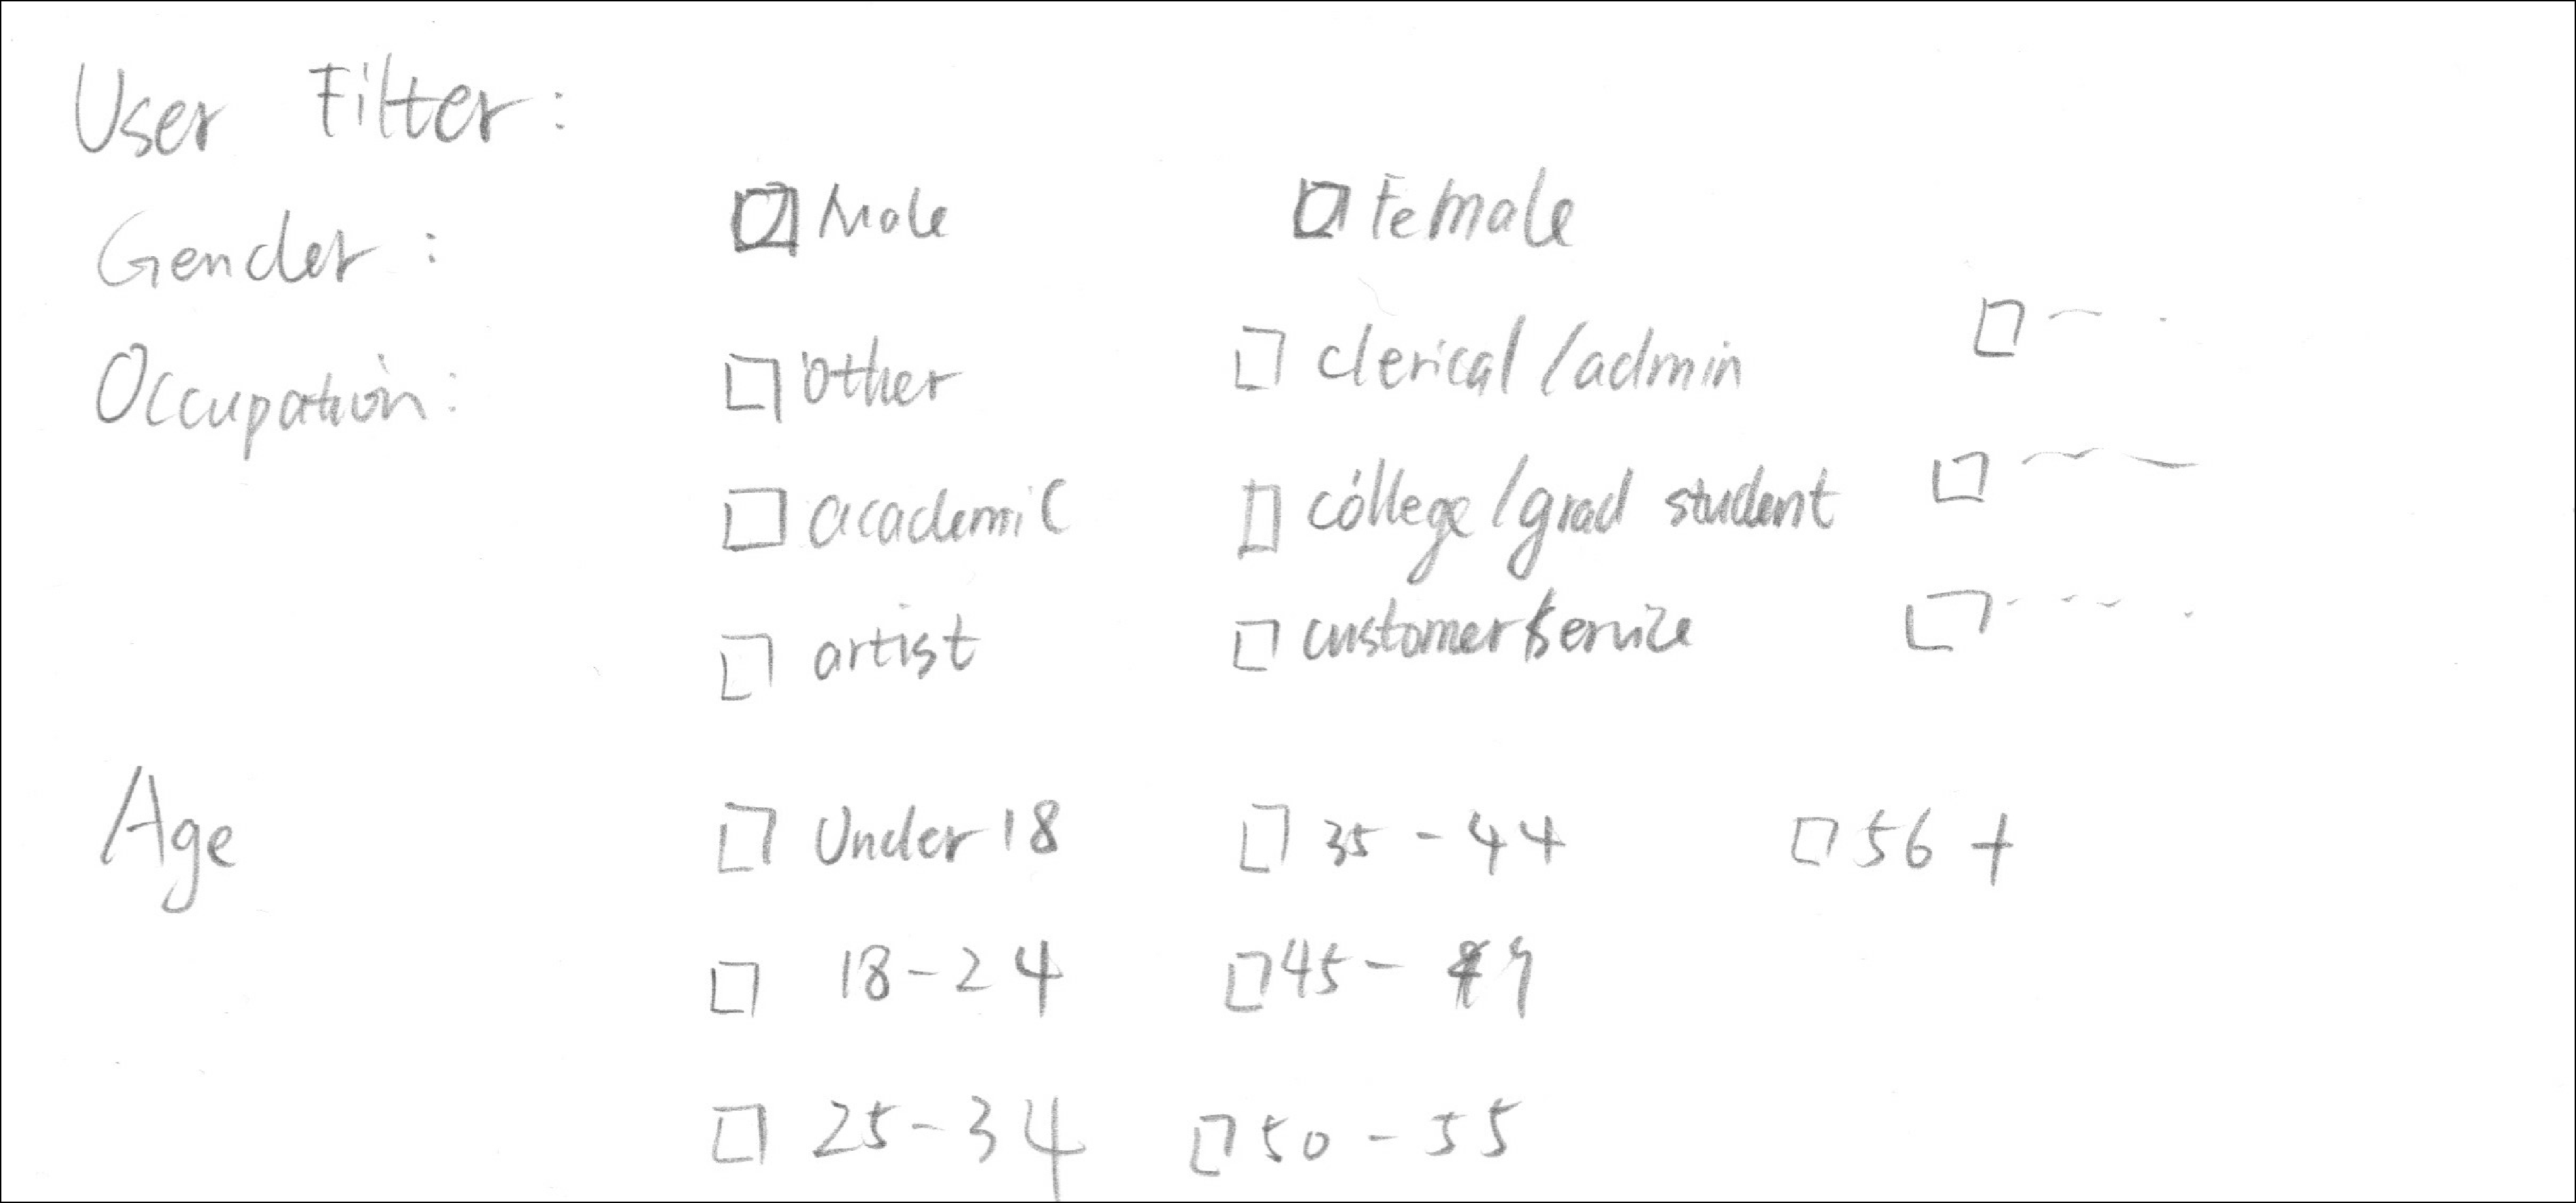
\includegraphics[width=.7\linewidth]{7.pdf}
}
\caption{Filter of user information}
\label{fig:fig7}
\end{figure}

\begin{figure}[h]
\centering{
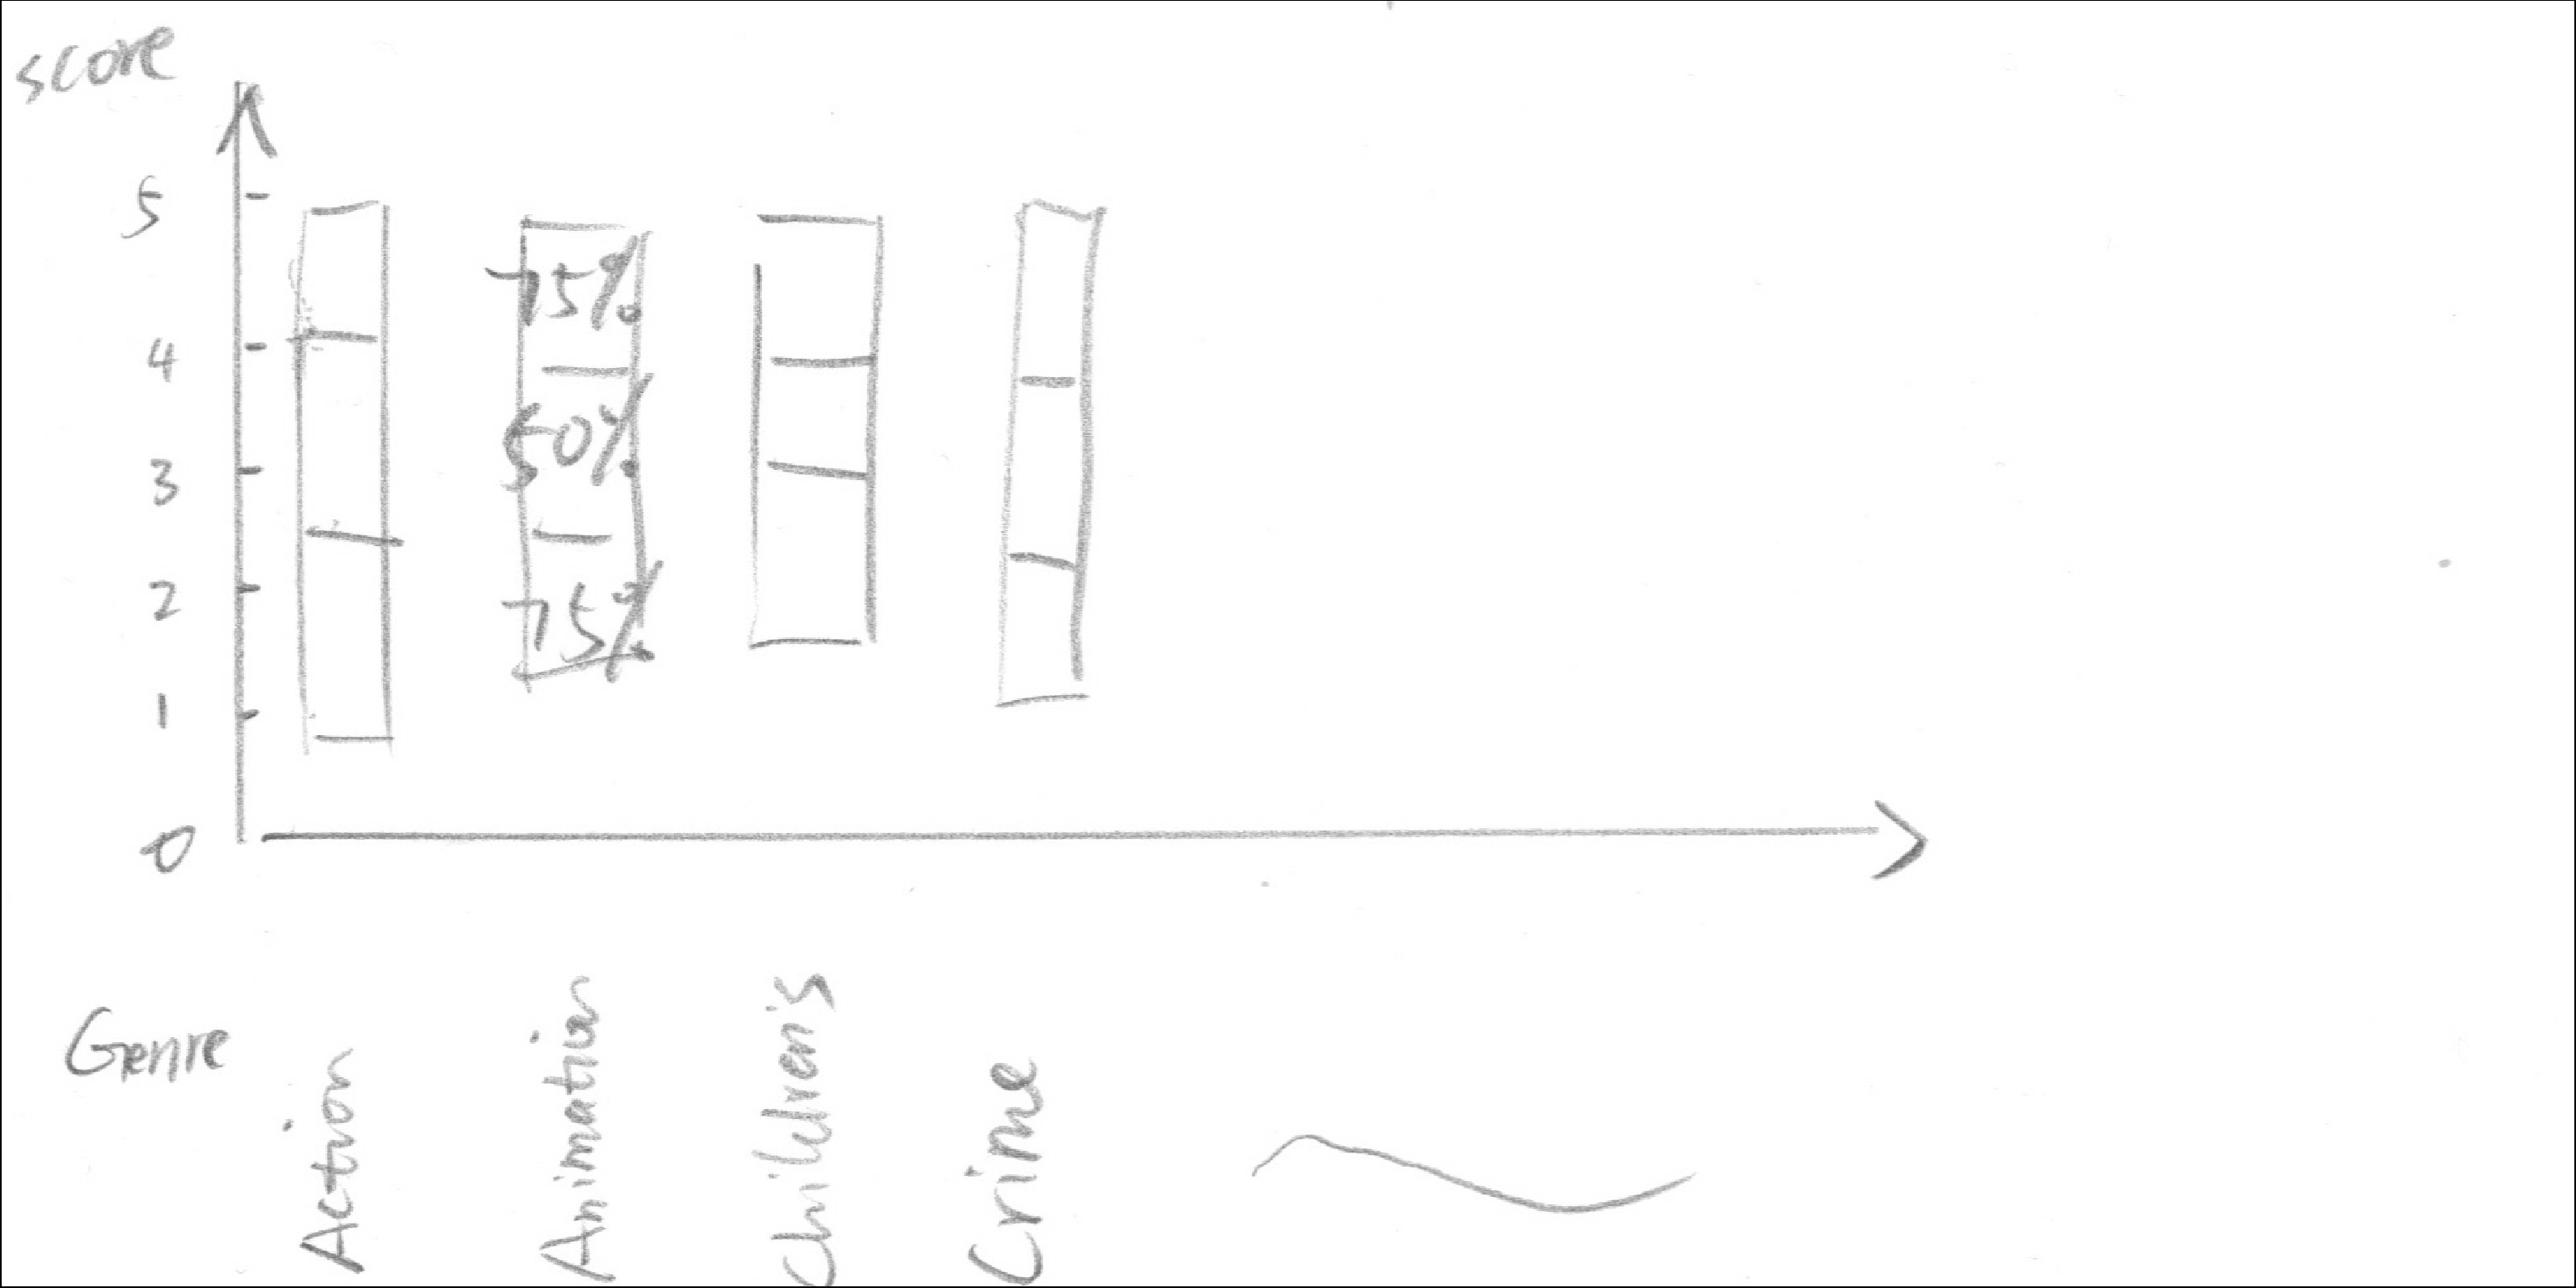
\includegraphics[width=.7\linewidth]{8.pdf}
}
\caption{Distributions of scores grouped by genres}
\label{fig:fig8}
\end{figure}

\begin{figure}[h]
\centering{
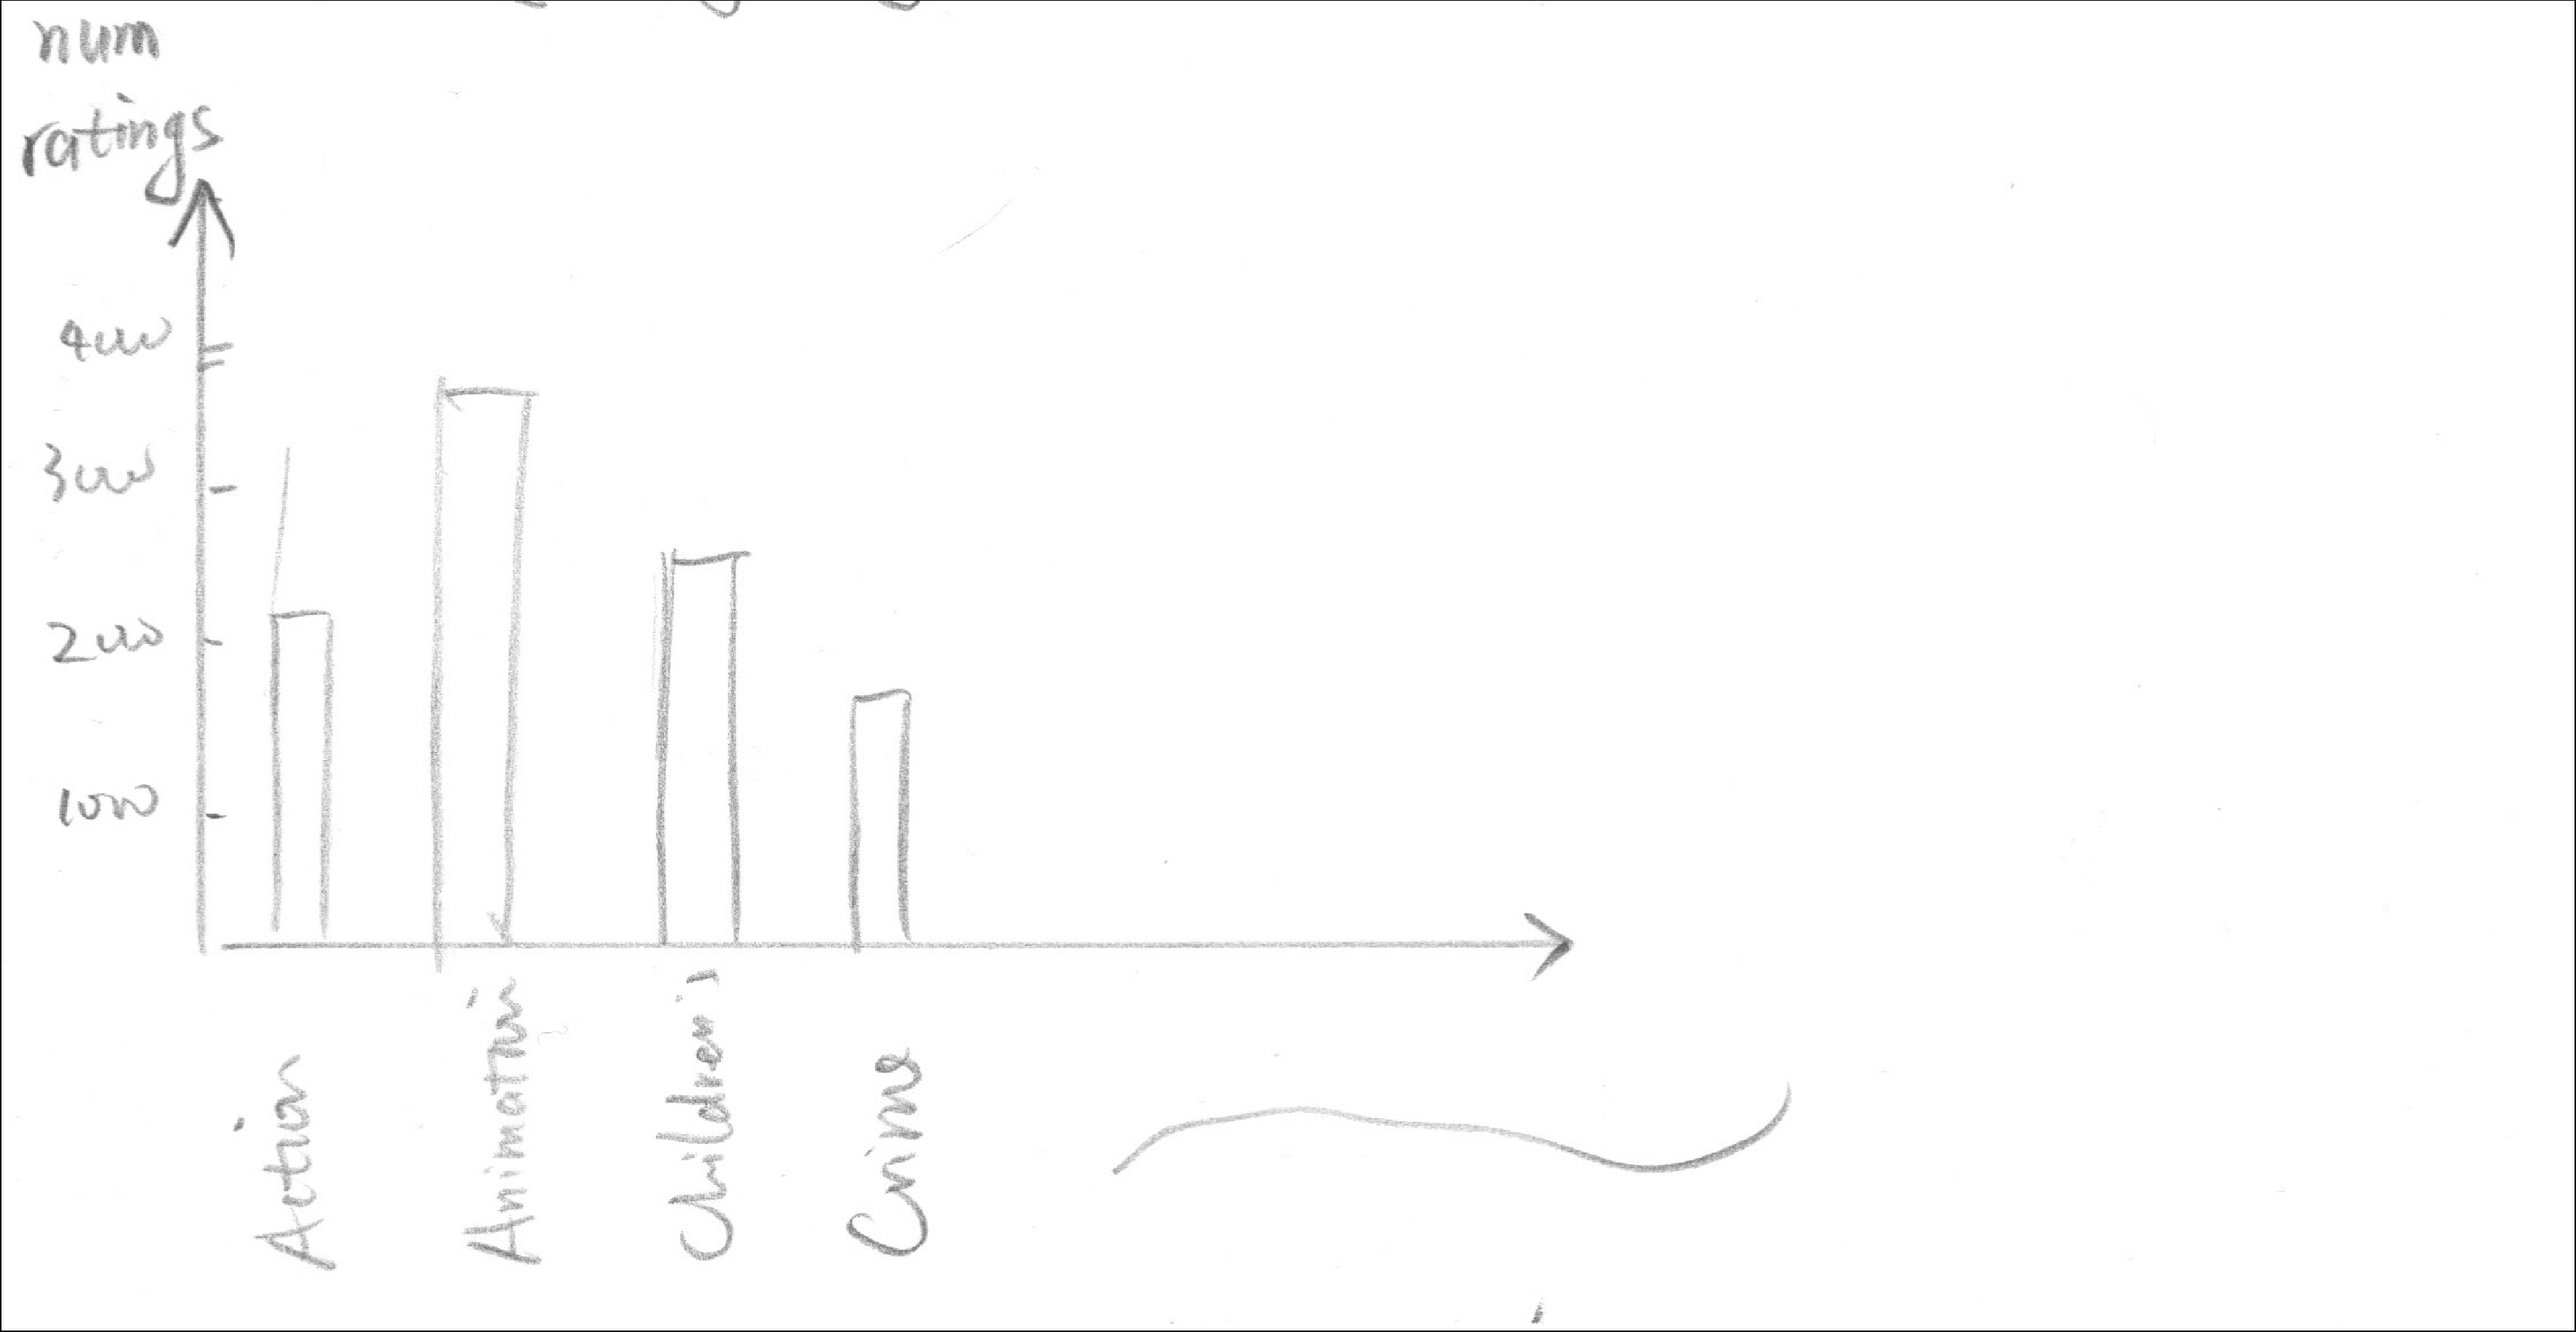
\includegraphics[width=.7\linewidth]{9.pdf}
}
\caption{Number of ratings grouped by genres}
\label{fig:fig9}
\end{figure}

\begin{figure}[h]
\centering{
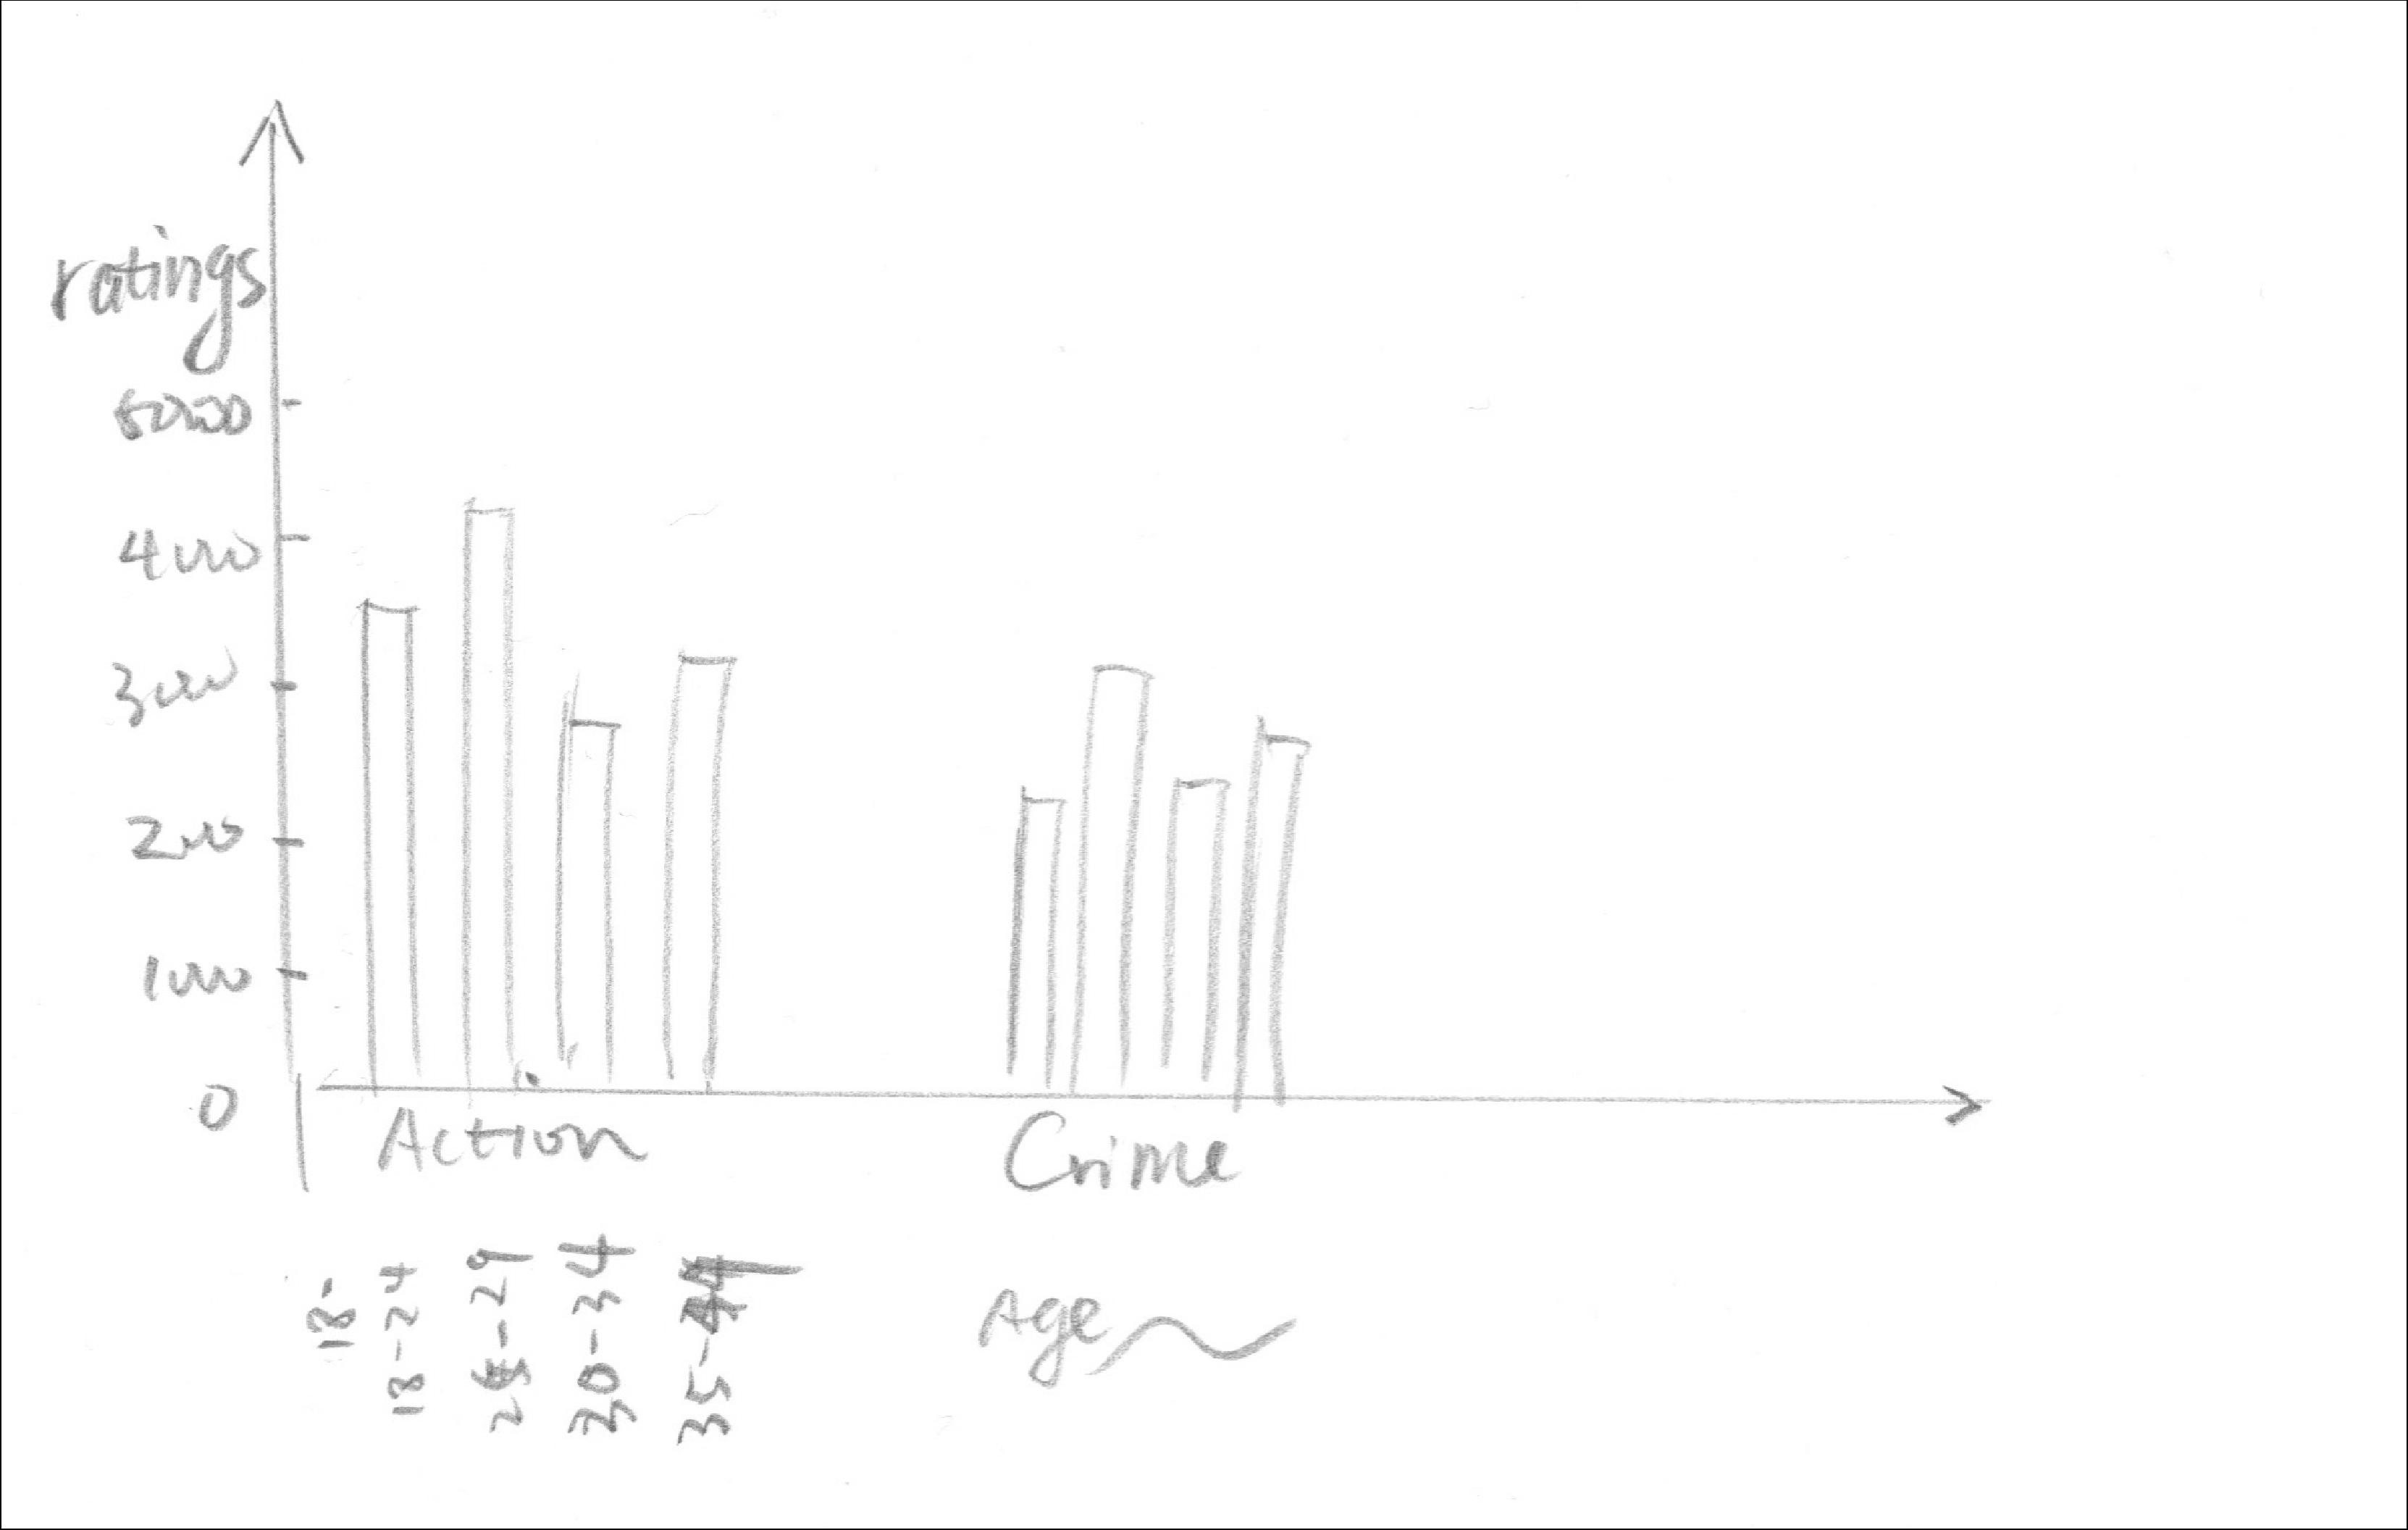
\includegraphics[width=.7\linewidth]{10.pdf}
}
\caption{Number of ratings grouped by genres and subdivided by ages}
\label{fig:fig10}
\end{figure}

\begin{figure}[h]
\centering{
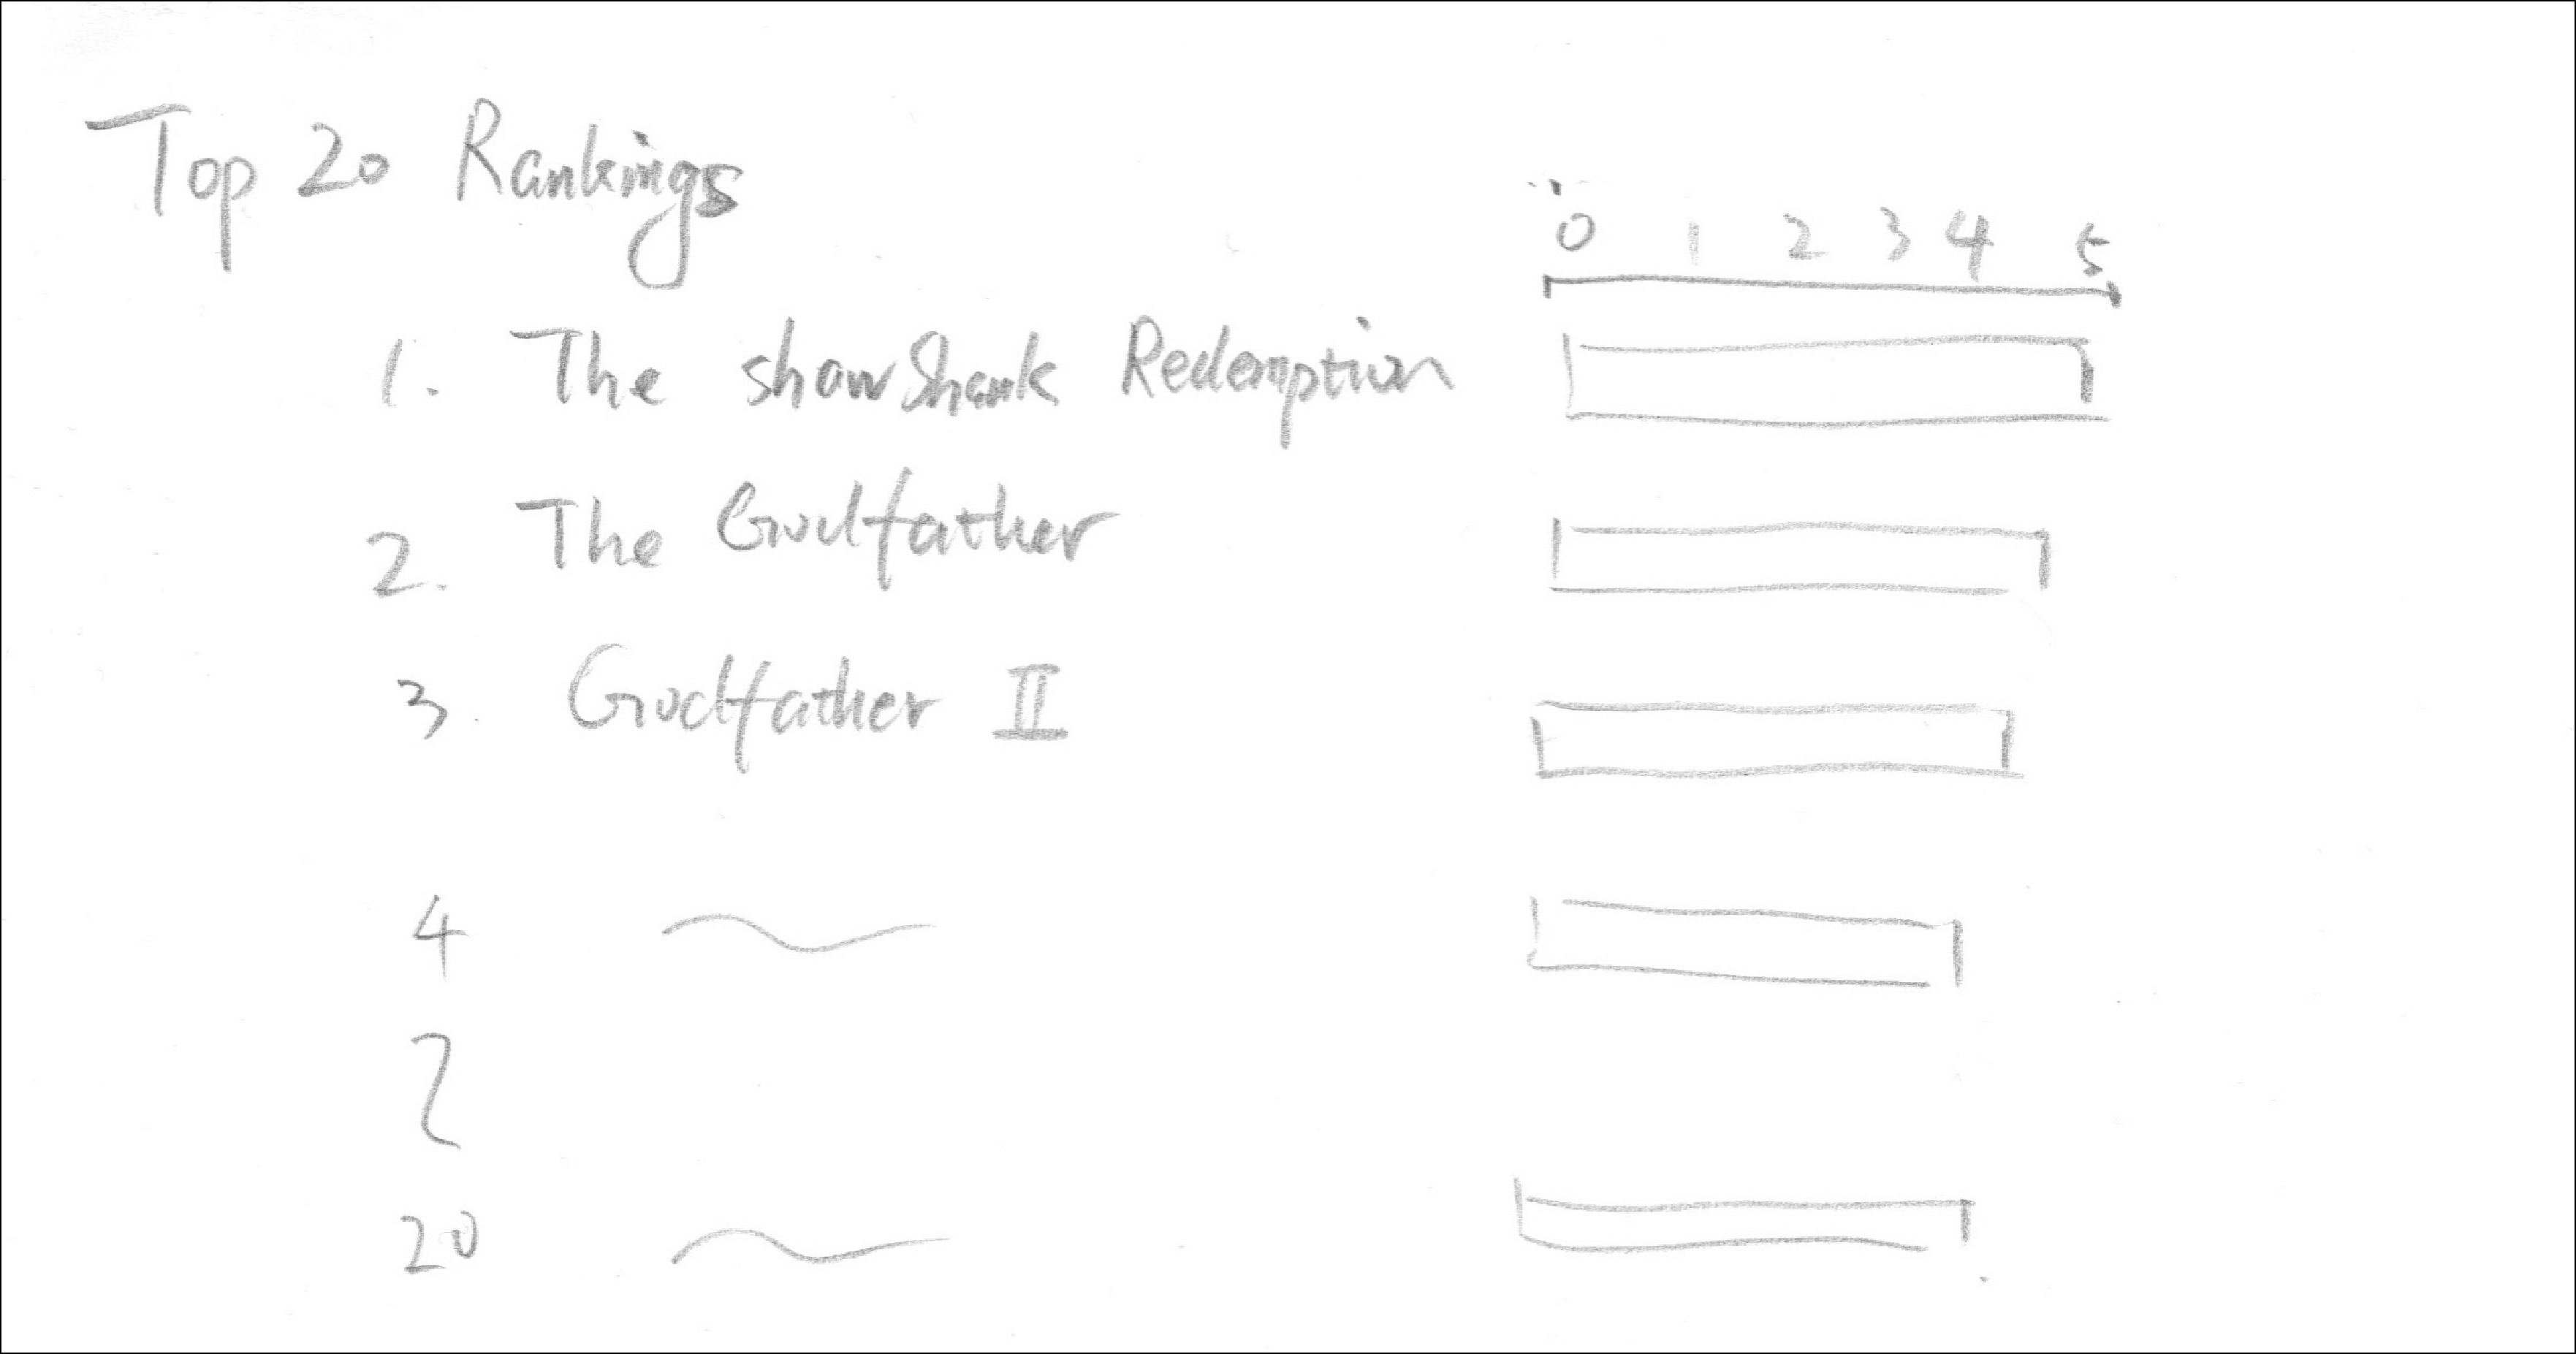
\includegraphics[width=.7\linewidth]{11.pdf}
}
\caption{Rankings of movie scores}
\label{fig:fig11}
\end{figure}

\begin{figure}[h]
\centering{
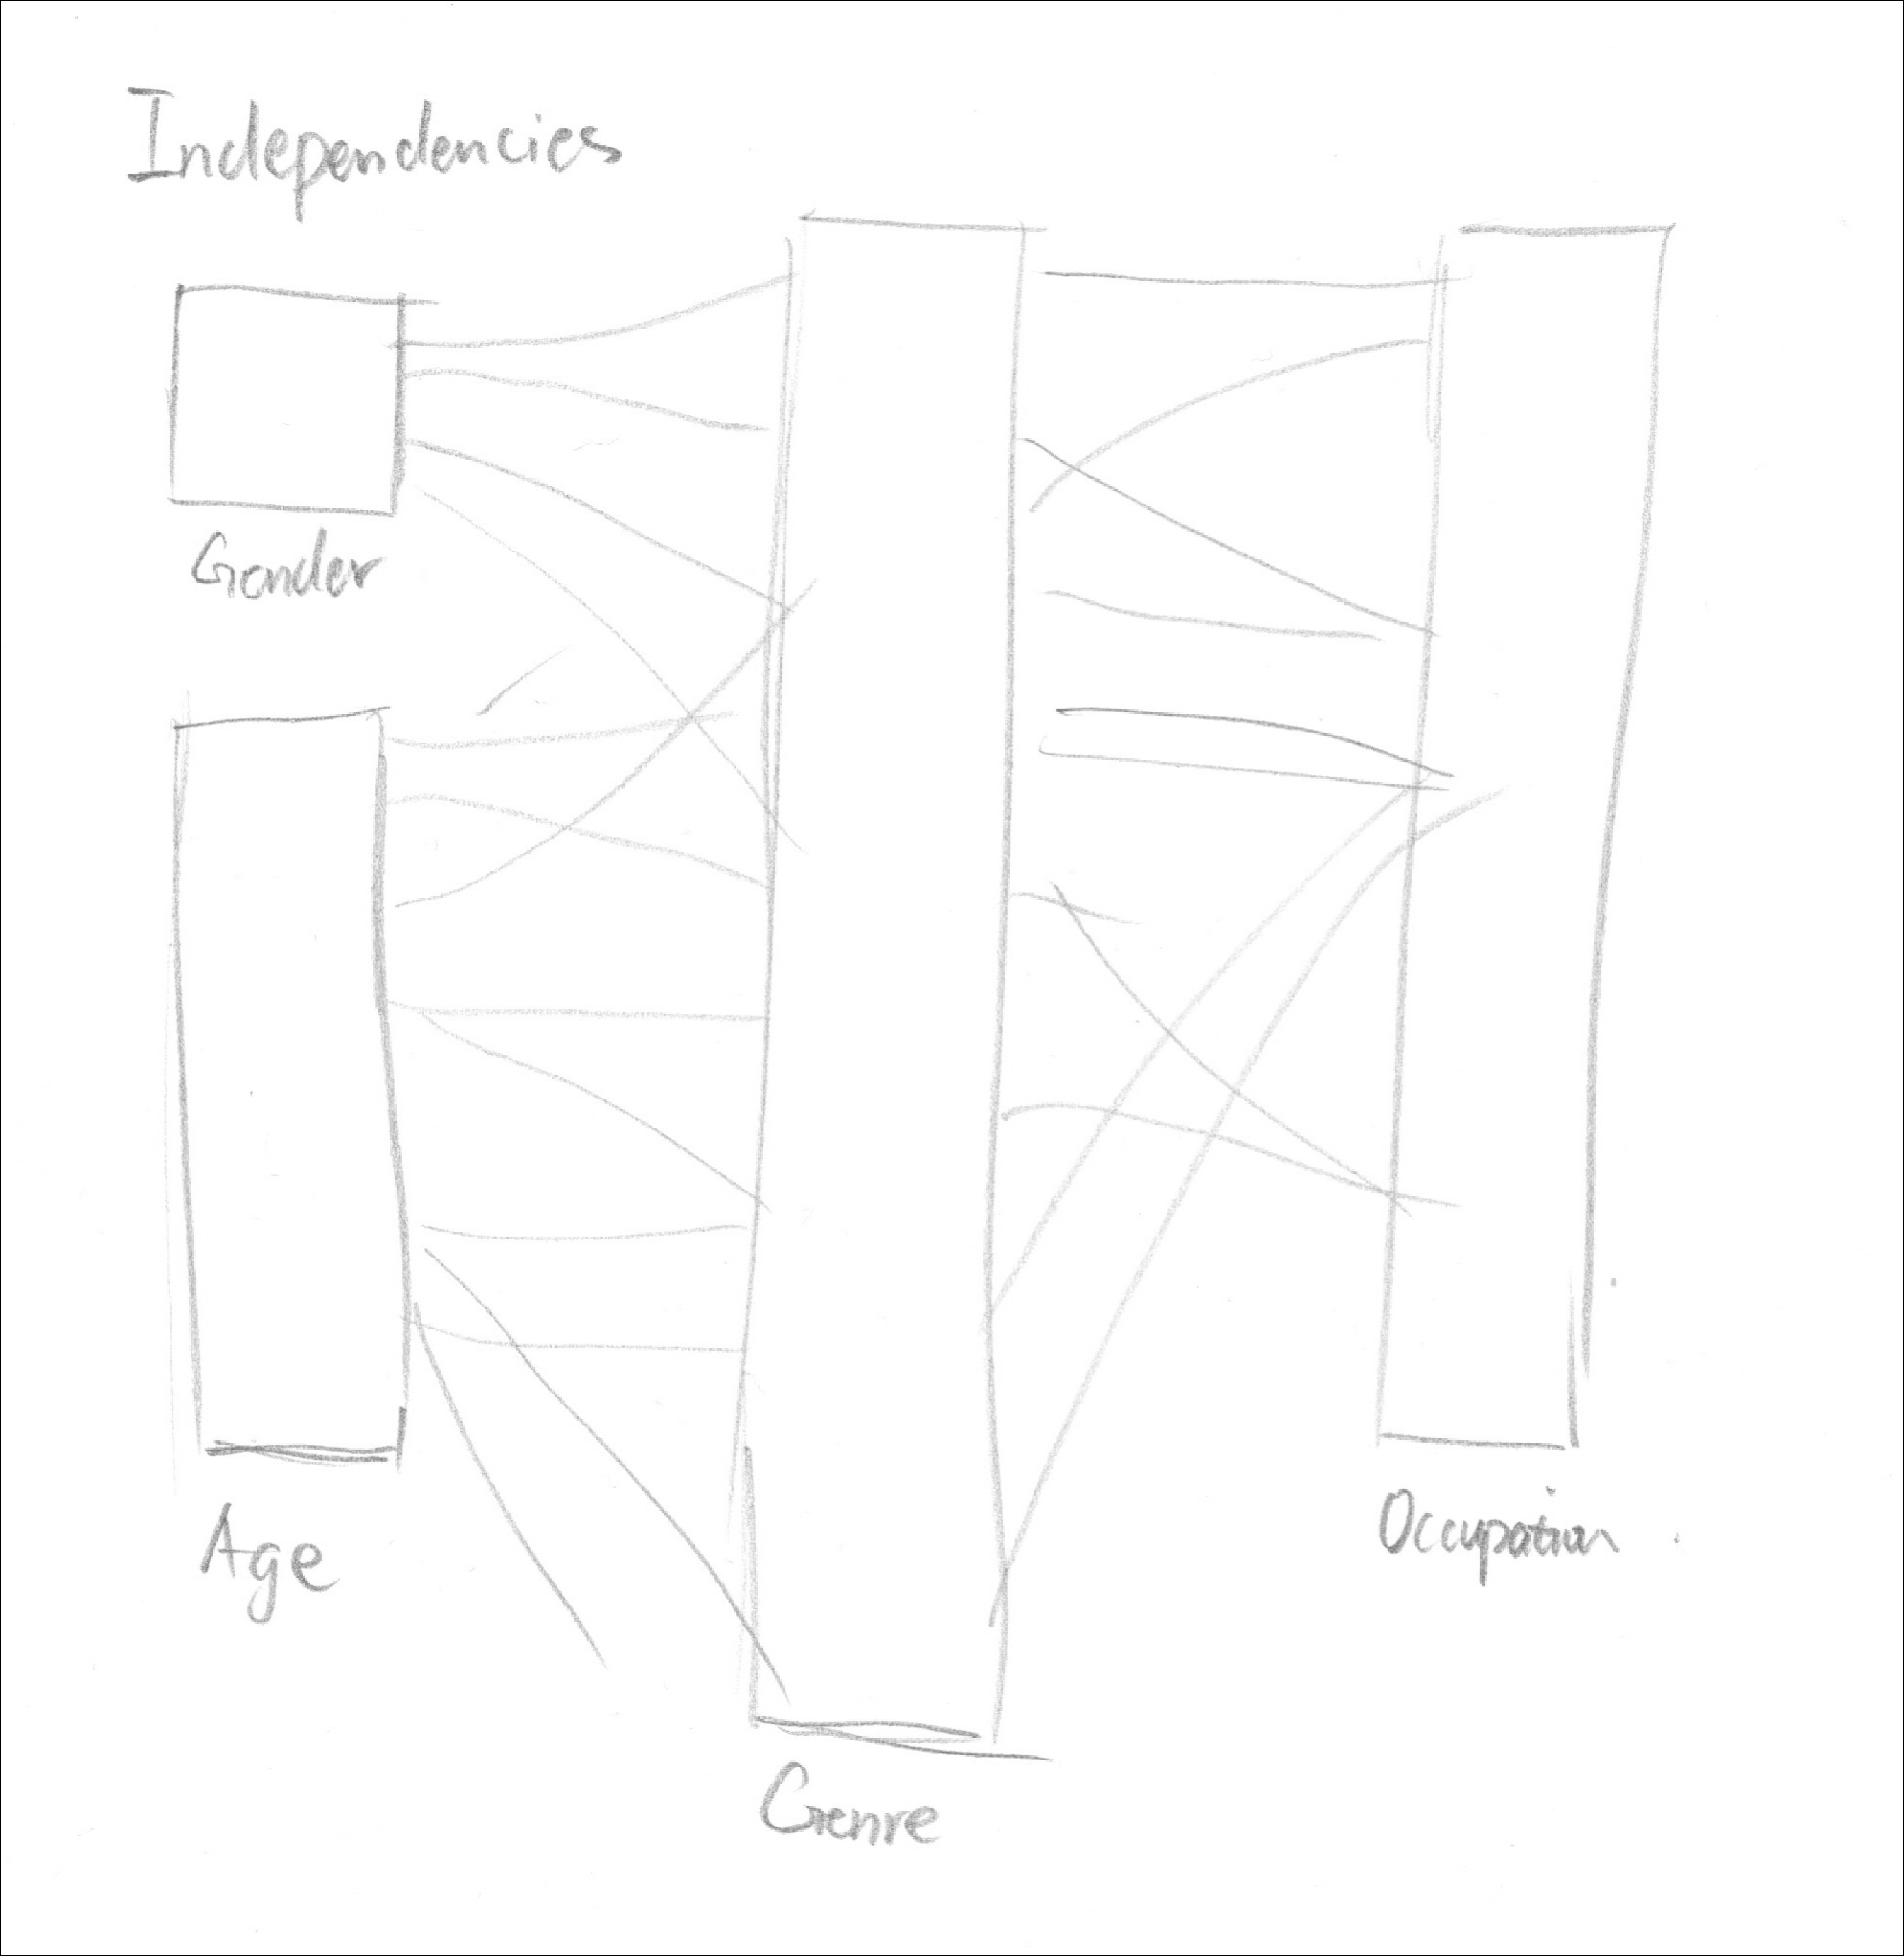
\includegraphics[width=.7\linewidth]{12.pdf}
}
\caption{Dependencies of users and movies}
\label{fig:fig12}
\end{figure}

\subsection{Our Design in Final Submission}

\subsubsection{Preview}

In our final design, we have tried some BI tools such as tableau and qlikview. Then we have some good ideas. We decide to build our visualization project into a concise, elegant and flexible tool. So we focus more on the interaction, and try not to display too many information in a single webpage. What information to be display is totally up to the user.

\subsubsection{Design}

The user could select any valid attribute for $x$ axis, $y$ axis and chart type. We have two views in our final design, one for user, and one for movie. In the user view, you can select a specific user, and his ratings of different movies will display. You can group these information in any attribute, and you can select number of records or average rating as $y$ axis. In the movie view, you can select a specific movie, and all users who have rated this movie will display. You can group these users into different attributes, such as age, state or sex. For details, please see Figure \ref{fig:fin_1}.

\begin{figure}[h]
\centering{
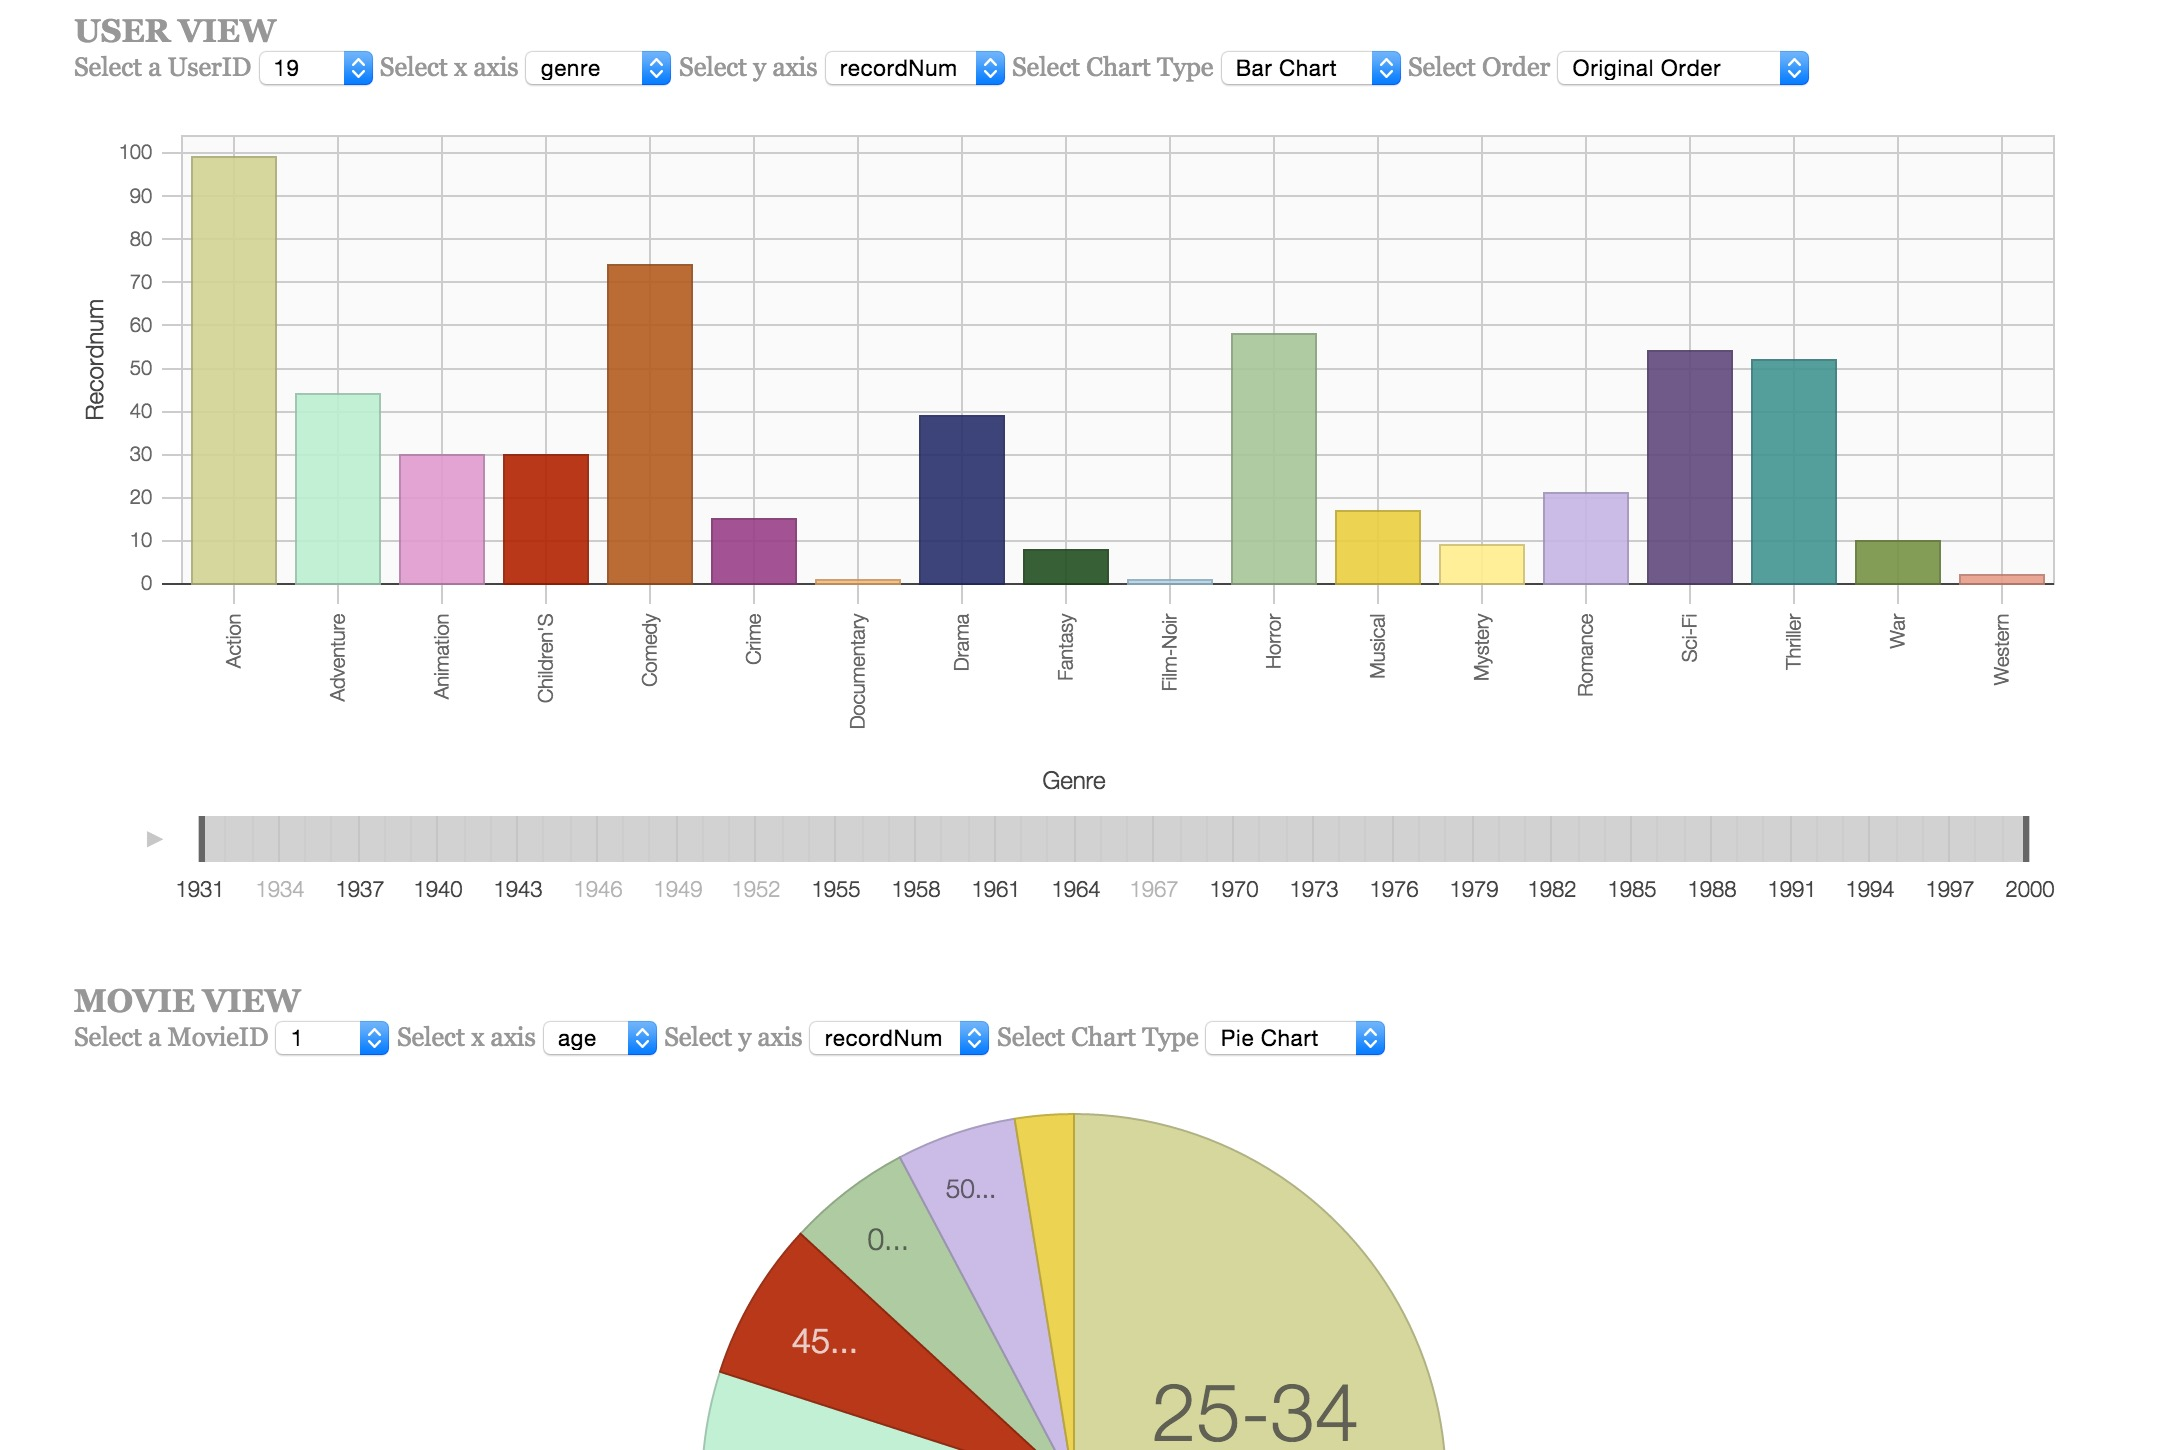
\includegraphics[width=.7\linewidth]{fin_1.png}
}
\caption{Design}
\label{fig:fin_1}
\end{figure}

\subsubsection{Validation of Attributes}

So first of all, we need to validate what attributes are valid for $x$ axis and $y$ axis. The categorical attributes are for $x$ axis, and numerical attributes are for $y$ axis. So in the user view, the categorical attributes are movieID, genre and released year. In the movie view, the categorical attributes could be age, state and sex. Both user view and movie share the same y-axis: number of records and average rating.


\subsubsection{Color}

We should color the categorical chart into different colors based on the selected id or selected group. For the numerical attributes, we should use the same hue and scale by saturation and lightness.


\subsubsection{Chart Type}

1. Bar Chart

Bar chart is the most flexible chart type, and it can be useful in any circumstance. We should implement it. And we need to provide sorting function for bar chart.


2. Tree Map and Pie Chart

Tree Map and Pie Chart are good charts to display proportion of different elements. So we should also include them both. However, the tree map and pie chart are only valid when y axis is set to number of records. The proportion is pointless when y axis is set to average rating.


3. Box plot

Box plot is also a very helpful tool to observe the distribution of rating. In the user view, when the x-axis is movieID, the box plot is the same as point chart because the record number is 1 for each group. In the case when x-axis is genre or year, the recordNum for different group may be larger than 1, so we can see the top tukey, first quartile, median, third quartile and bottom tukey. The box plot is pointless when y axis is set to recordNum. For details, please see Figure \ref{fig:fin_2}.

\begin{figure}[h]
\centering{
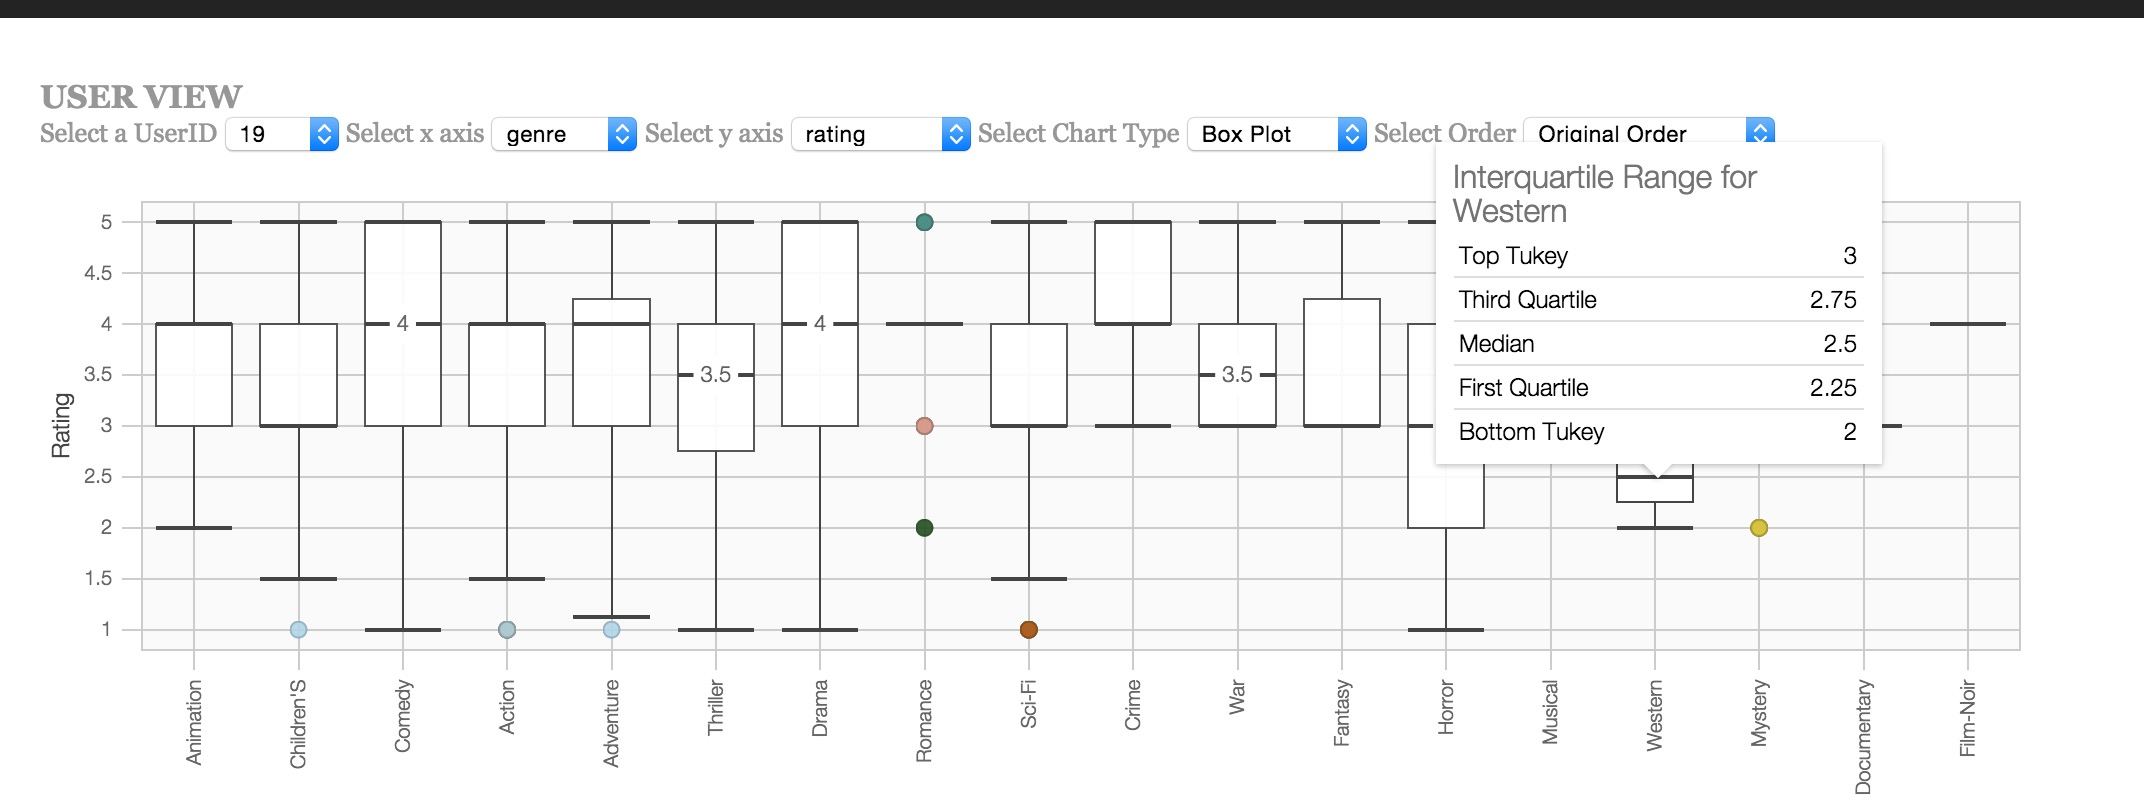
\includegraphics[width=.7\linewidth]{fin_2.png}
}
\caption{Dependencies of users and movies}
\label{fig:fin_2}
\end{figure}


4. Geography Map

Since we have postal code information in the user information, we can display the location distribution information as geo map in the movie view. You can see different the recordNum or average rating of different states in US. We use color to scale the numberical attributes in geo map.


5. Network Chart

Network Chart is a powerful tool. We have taken this type into consideration, but we at last abandon this chart, because there are over 6000 users and 3000 movies and 1 million ratings in the dataset, it's almost impossible to display all the information in a network chart...


6. Point Chart

We also include a point chart in our design. It's also very flexible.

\subsubsection{Selection of attributes and charts}

We use dropdown menu list to select attributes, and we also need to validate the relationship between attributes and charts. For example, if you select recordNum as $y$ axis, you could not select box plot. If you select rating as $y$ axis, you could not select pie chart and tree map.

{\bf Interaction}

1. Drop down menu

You can select any valid attributes for $x$ axis and $y$ axis and bar chart.

2. Tooltip

With the help of tooltip, we can see more information we want when we move mouse over the element in the chart.


3. Timeline

In the user view, we can user timeline to filter out the movie released in a time range. If we can display the evolution of information over time, that'll be better.


4. Zoom in and zoom out

In the movie view, when you select ``state'' as $x$ axis and ``geo map'' as chart type, it will show a us geo map. We can zoom in and zoom out for more details.


5. Sort

When chosen bar chart, you can sort the elements in the chart.


\section{Implementation}

\subsection{Data Preprocessing}

We simply transformed the original data into the format that can be easily processed. Then we imported the transformed data into MySQL. We used three tables to present the transformed data. The SQL statement ``Create table if not exists User( UserID int, Gender int, Age int, Occupation int, ZipCode varchar(15) )'' can create User table. The SQL statement ``Create table if not exists Movie( MovieID int, Title varchar(100), Year int, Genres varchar(50) )'' can create Movie table. The SQL statement ``Create table if not exists Rating( UserID int, MovieID int, Rating int, Timestamp varchar(15) )'' can create Rating table. After inserting the tuples into the tables in the database, we can easily gain some statistics by performing the corresponding aggregate queries.

We perform our offline data analysis by using both of SQL queries and Java programming. The advantage of performing SQL queries is that we can use only one statement to generate the file that contains the aggregation information we need. For example, if we want to find the average rating for all the movies in a specific year, we can just perform such a SQL statement ``select m.year as Year, avg(r.rating) as AverageRating, count(*) as RecordNum from (select distinct movieid, year from movie) as m, (select movieid, rating from rating) as r where m.movieid = r.movieid group by m.Year''. If we want to find the average rating for all the movies sharing a specific genre, we can just perform such a SQL statement ``select m.Genres as Genre, avg(r.rating) as AverageRating, count(*) as RecordNum from (select movieid, genres from movie) as m, (select movieid, rating from rating) as r where m.movieid = r.movieid group by m.Genres''. However, since there are only three tables in the database, the disadvantage of performing SQL queries is that it really needs some time to generate the final results by joining multiple tables. In fact, we have ever tried to perform an online interactive data analysis during visualization by connecting our JavaScript code to MySQL server. However, since performing join queries on such three tables really needs much time, we gave up the idea.

We can also use Java programming to perform offline data analysis. It can efficiently avoid the time cost of performing SQL queries. In fact, here we use Java programming to answer all kinds of complicated questions that we have proposed before and generate the related files.

\subsection{Visualization Implementation}

\subsubsection{Bar Chart}

As we can see, we select movieID as x Axis, we display rating information in barchart, and we can view the movie title, year in the tool tip. We can sort the bar in original, ascending or descending order. We can use timeline widget to filter out the movies. For details, please see Figure \ref{fig:fin_3} and Figure \ref{fig:fin_4}.

\begin{figure}[h]
\centering{
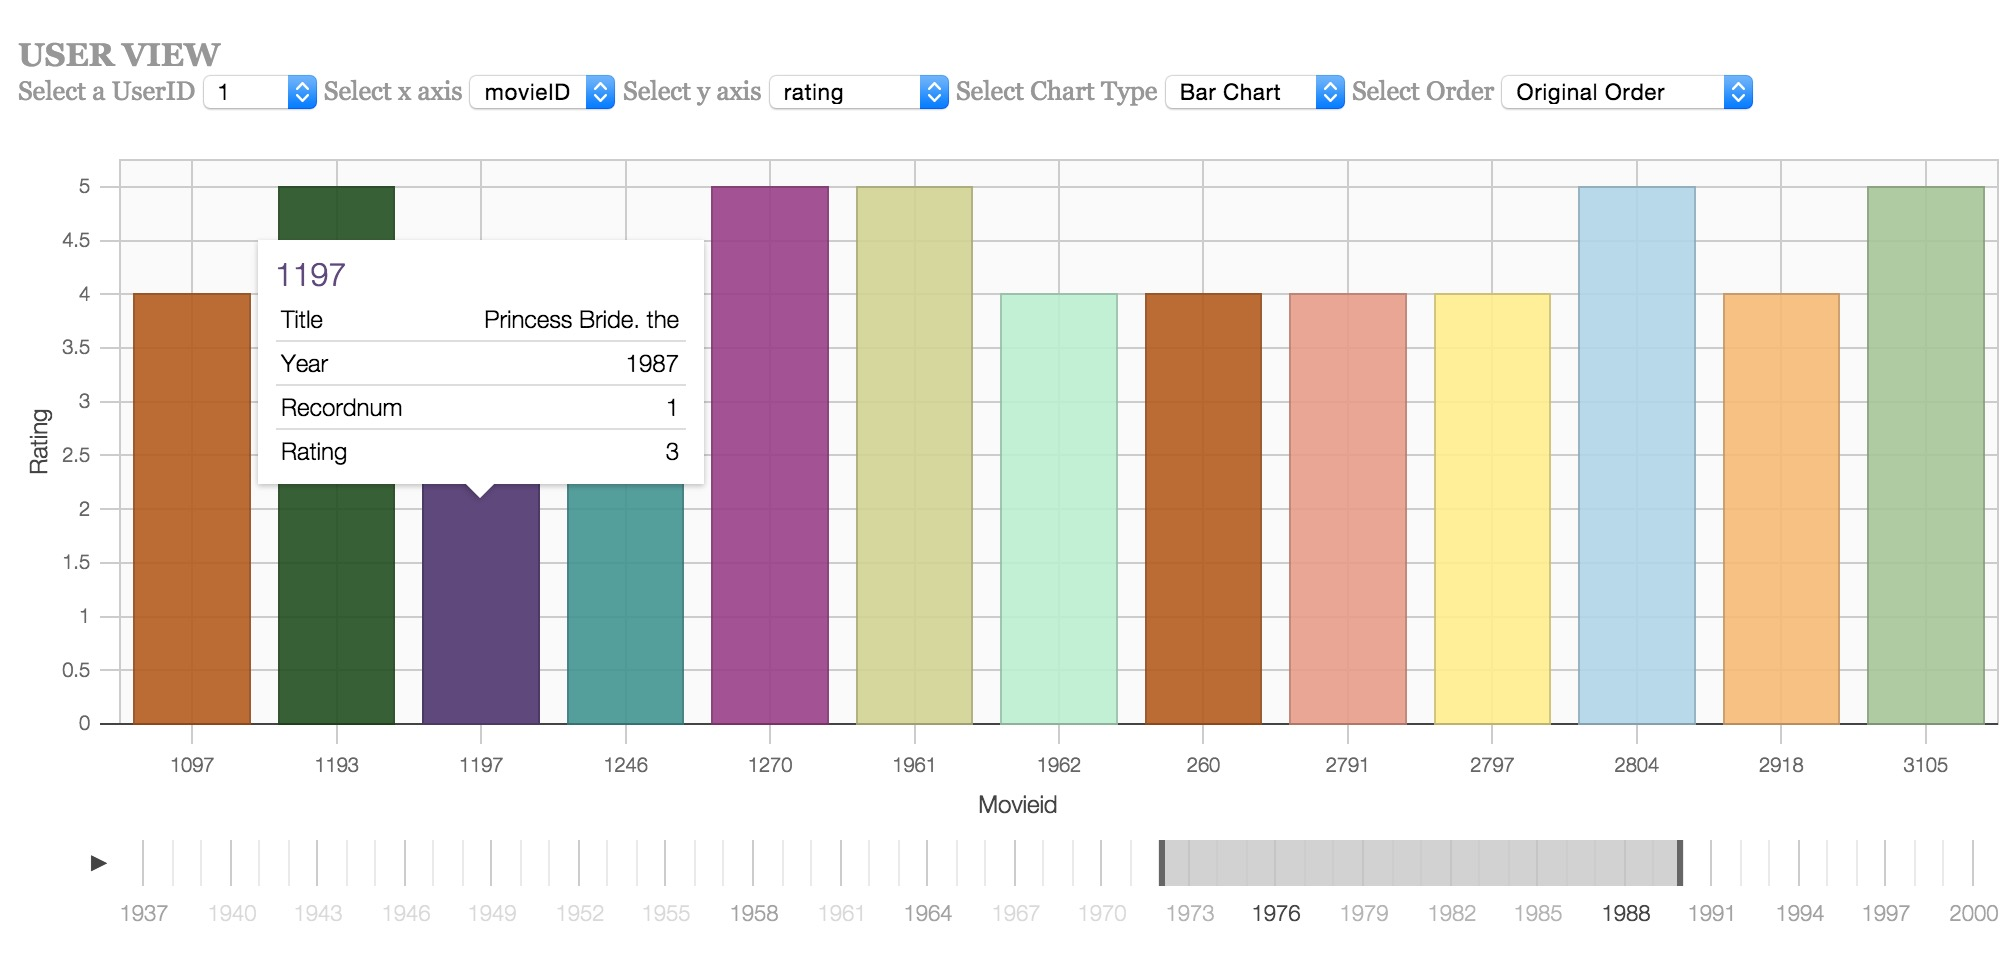
\includegraphics[width=.7\linewidth]{fin_3.png}
}
\caption{Dependencies of users and movies}
\label{fig:fin_3}
\end{figure}

\begin{figure}[h]
\centering{
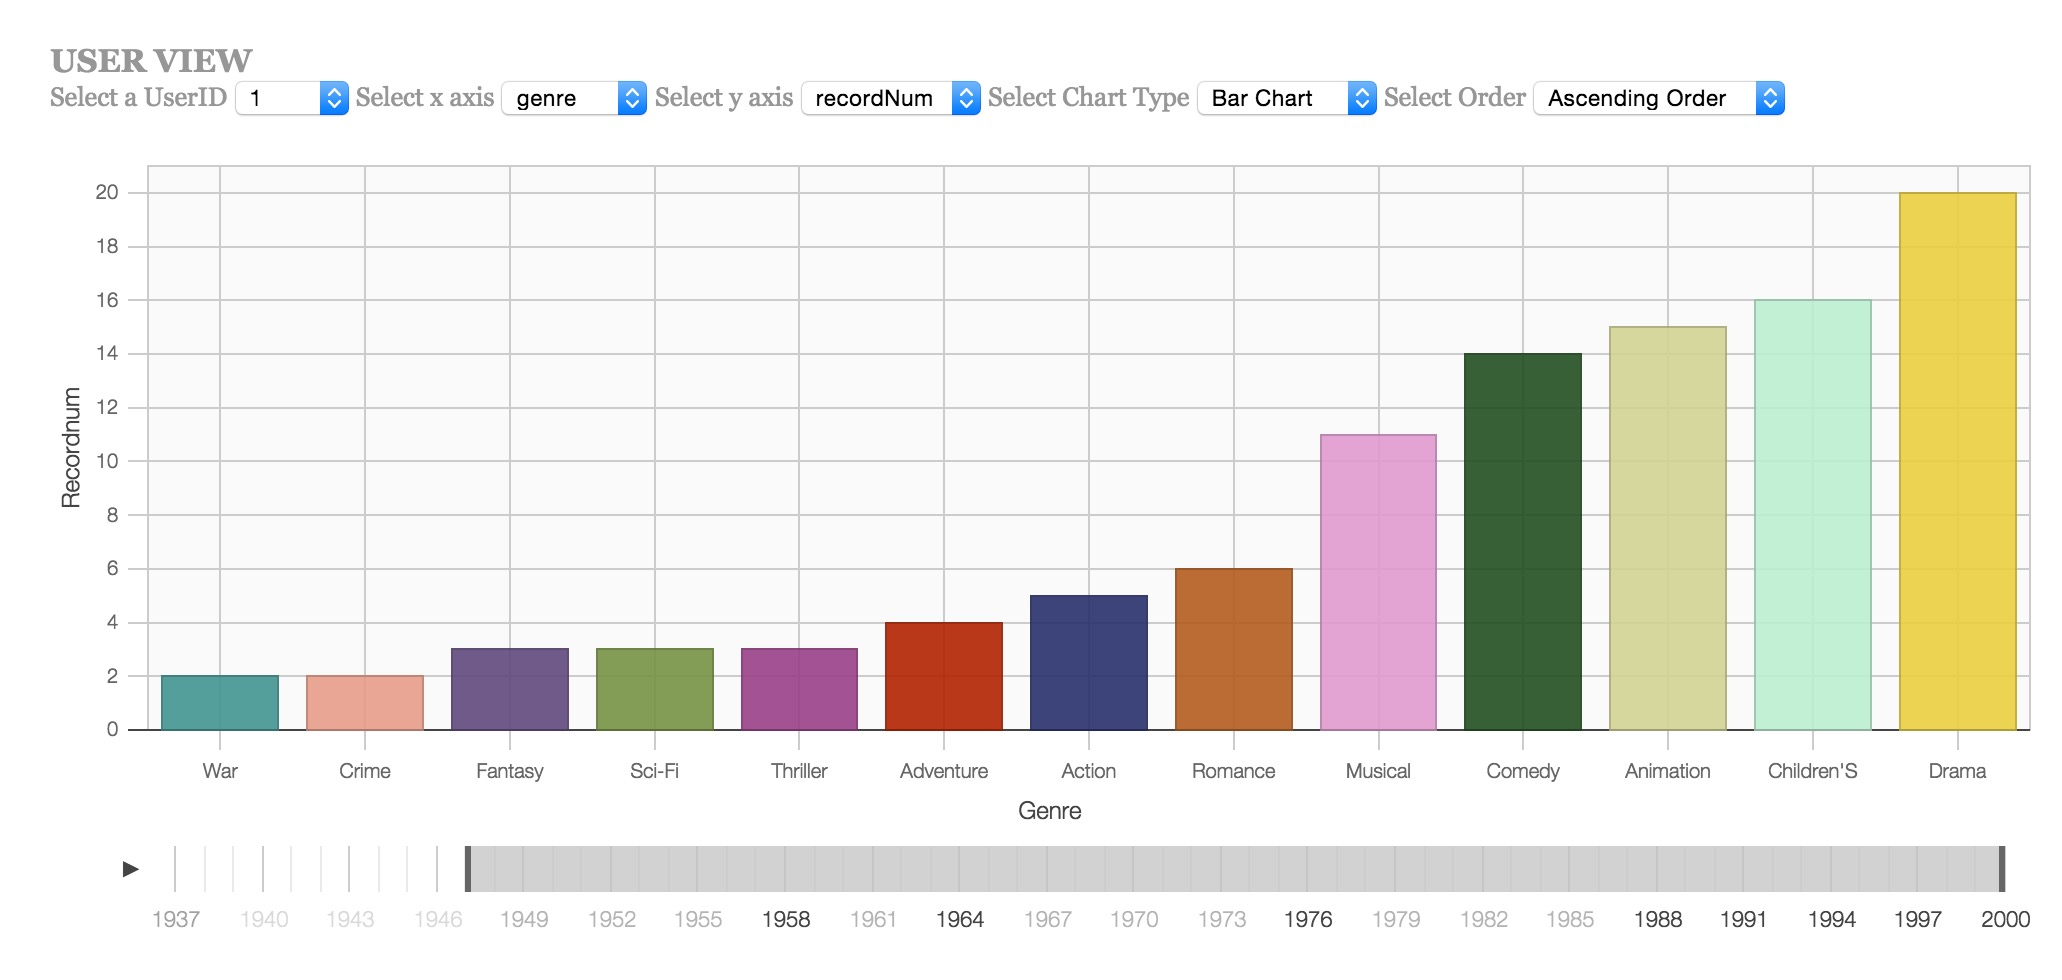
\includegraphics[width=.7\linewidth]{fin_4.png}
}
\caption{Dependencies of users and movies}
\label{fig:fin_4}
\end{figure}

\subsubsection{Box Plot}

When selected rating as y Axis, we can display the information by box plot. For details, please see Figure \ref{fig:fin_5}.

\begin{figure}[h]
\centering{
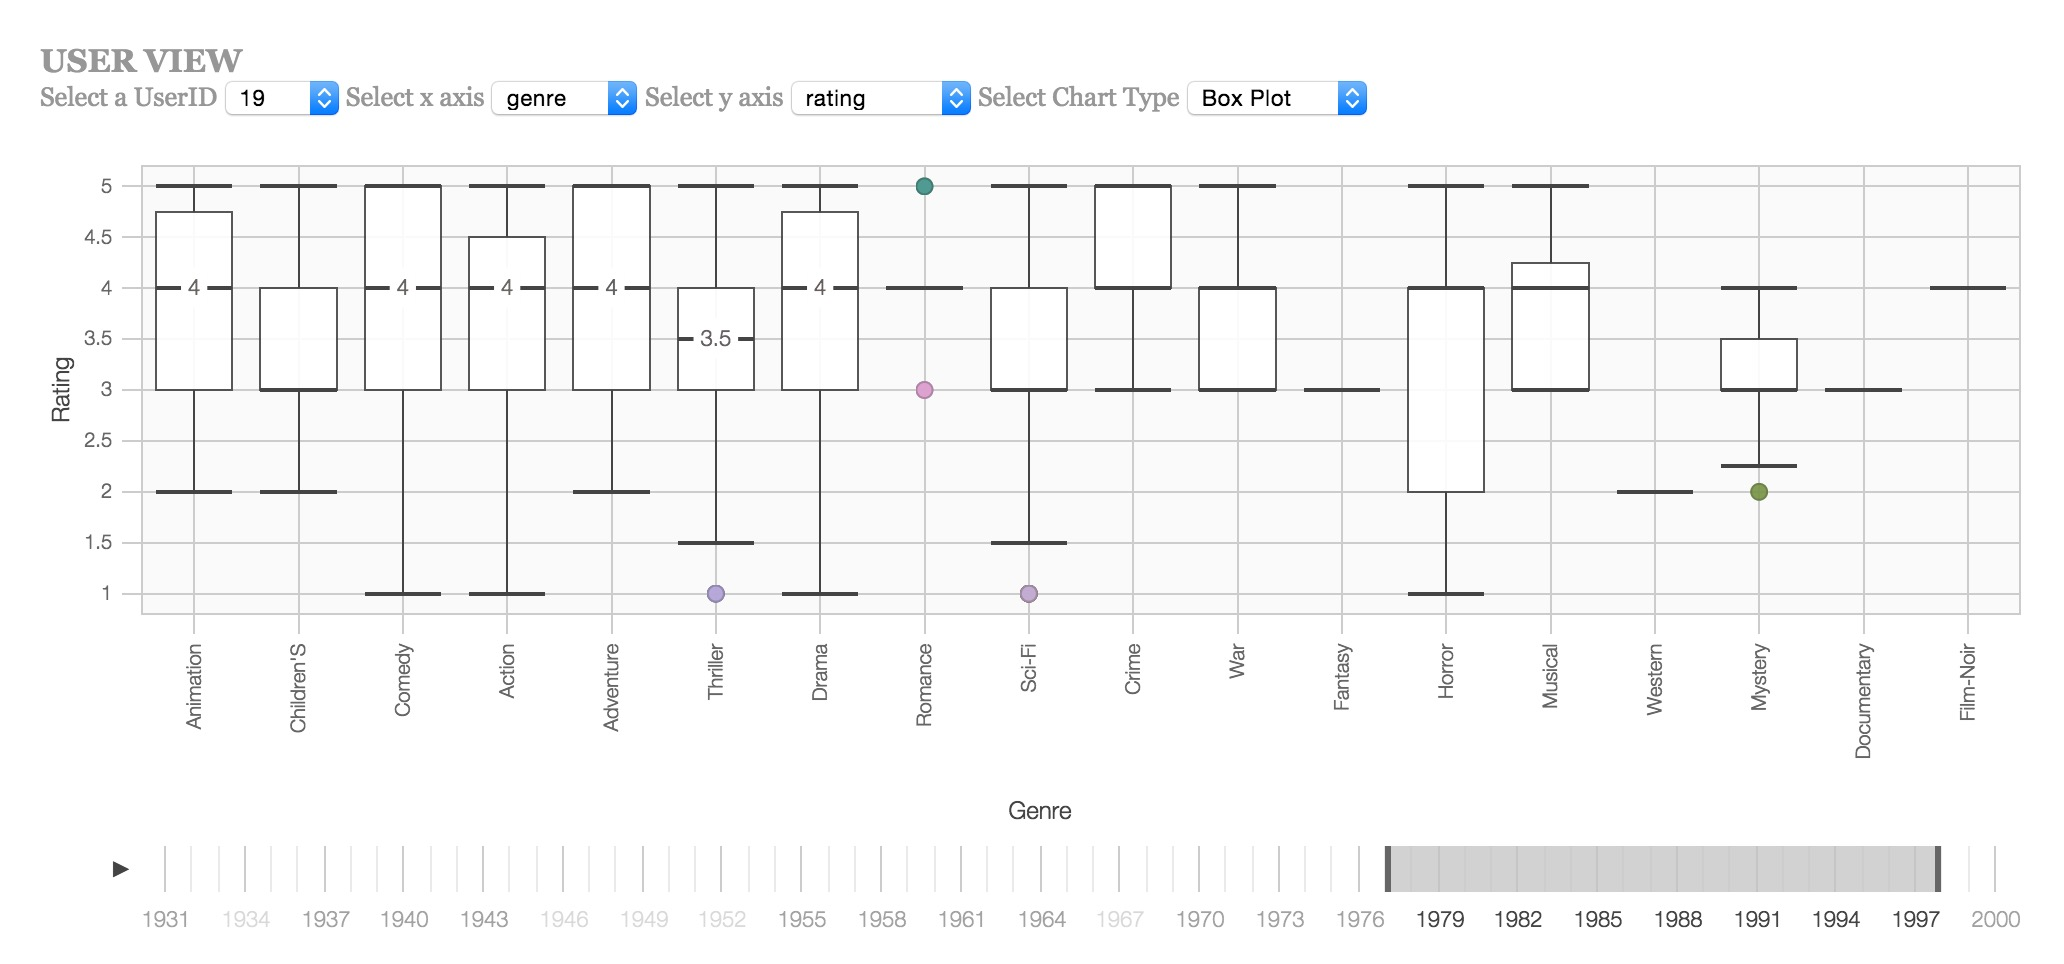
\includegraphics[width=.7\linewidth]{fin_5.png}
}
\caption{Dependencies of users and movies}
\label{fig:fin_5}
\end{figure}

\subsubsection{Point Chart}

The point chart is shown below. We have also implemented a strong feature: when you move mouse over a point, it can map the point to the left axis. Also tooltips included. For details, please see Figure \ref{fig:fin_6}.

\begin{figure}[h]
\centering{
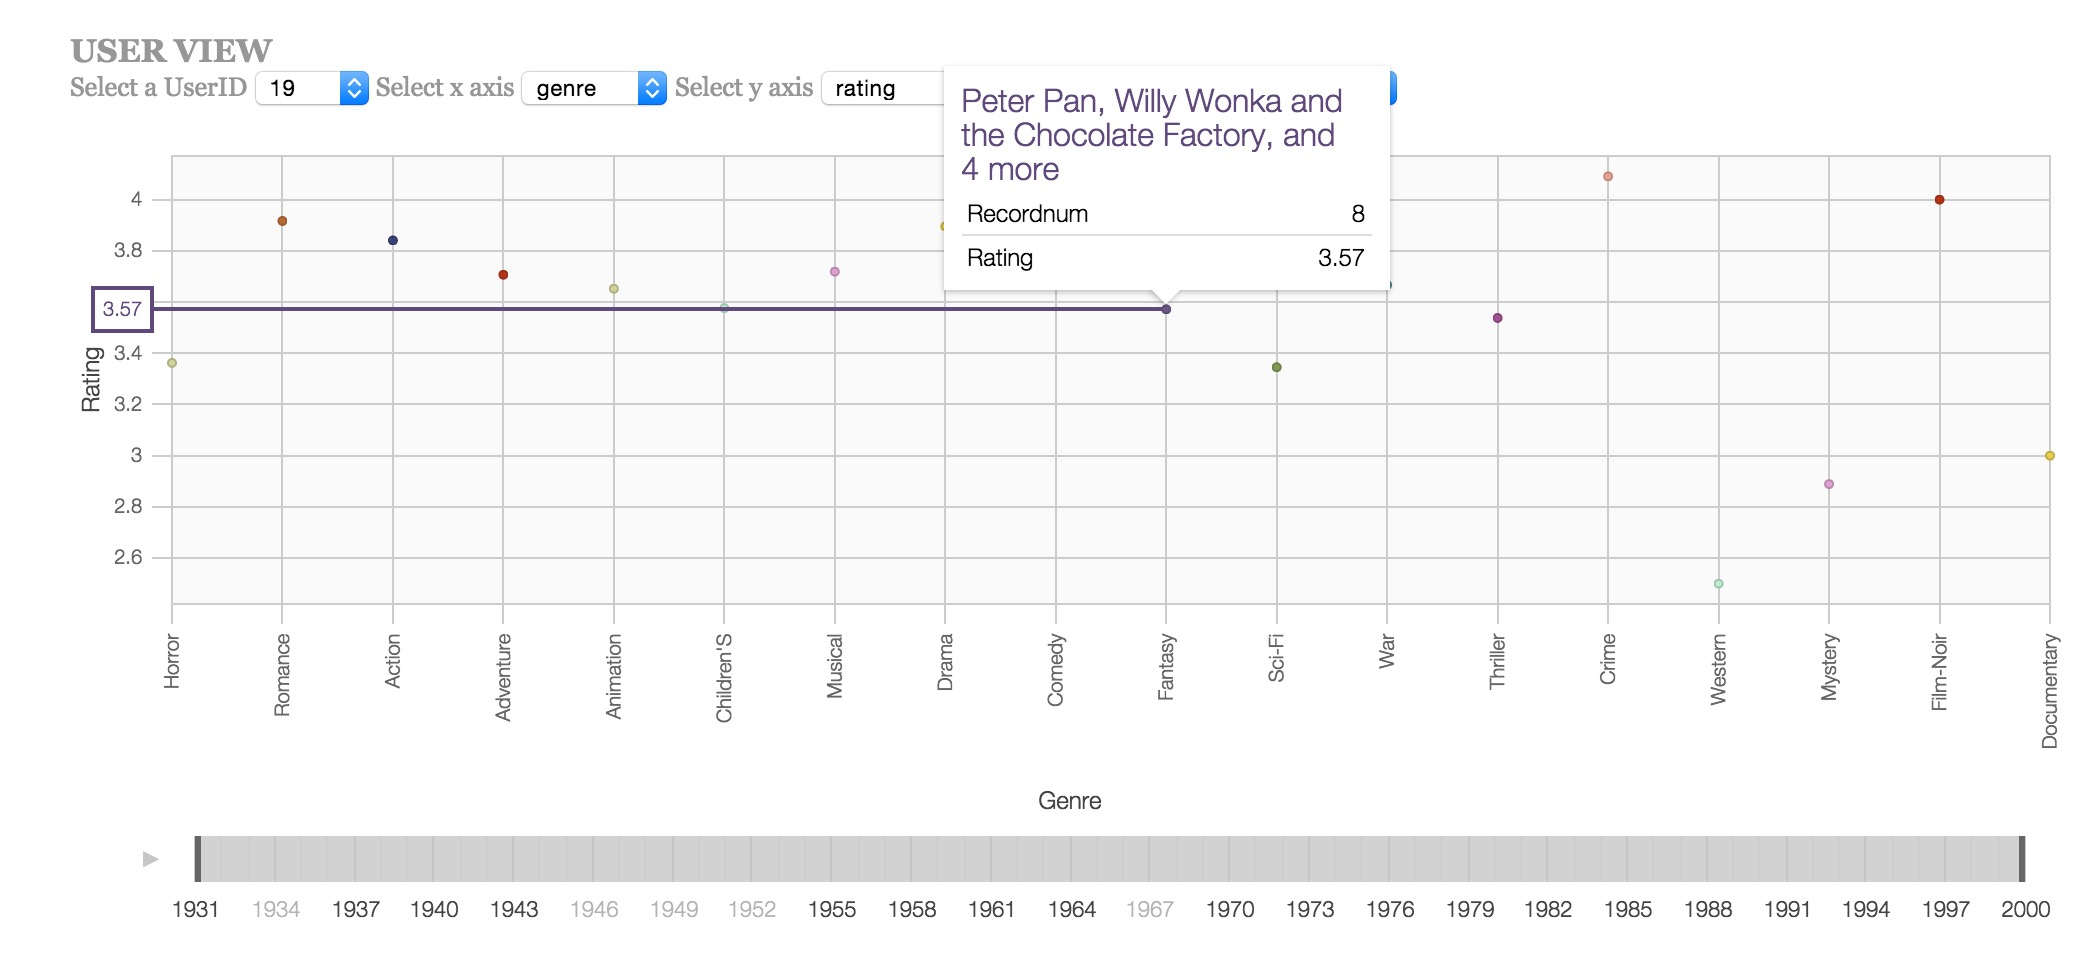
\includegraphics[width=.7\linewidth]{fin_6.png}
}
\caption{Dependencies of users and movies}
\label{fig:fin_6}
\end{figure}


\subsubsection{Tree Map and Pie Chart}

When selected recordNum as y Axis, we can use tree map and pie chart. From the below figure we can see that userID 19 watches Action movie the most. For details, please see Figure \ref{fig:fin_7} and Figure \ref{fig:fin_8}.

\begin{figure}[h]
\centering{
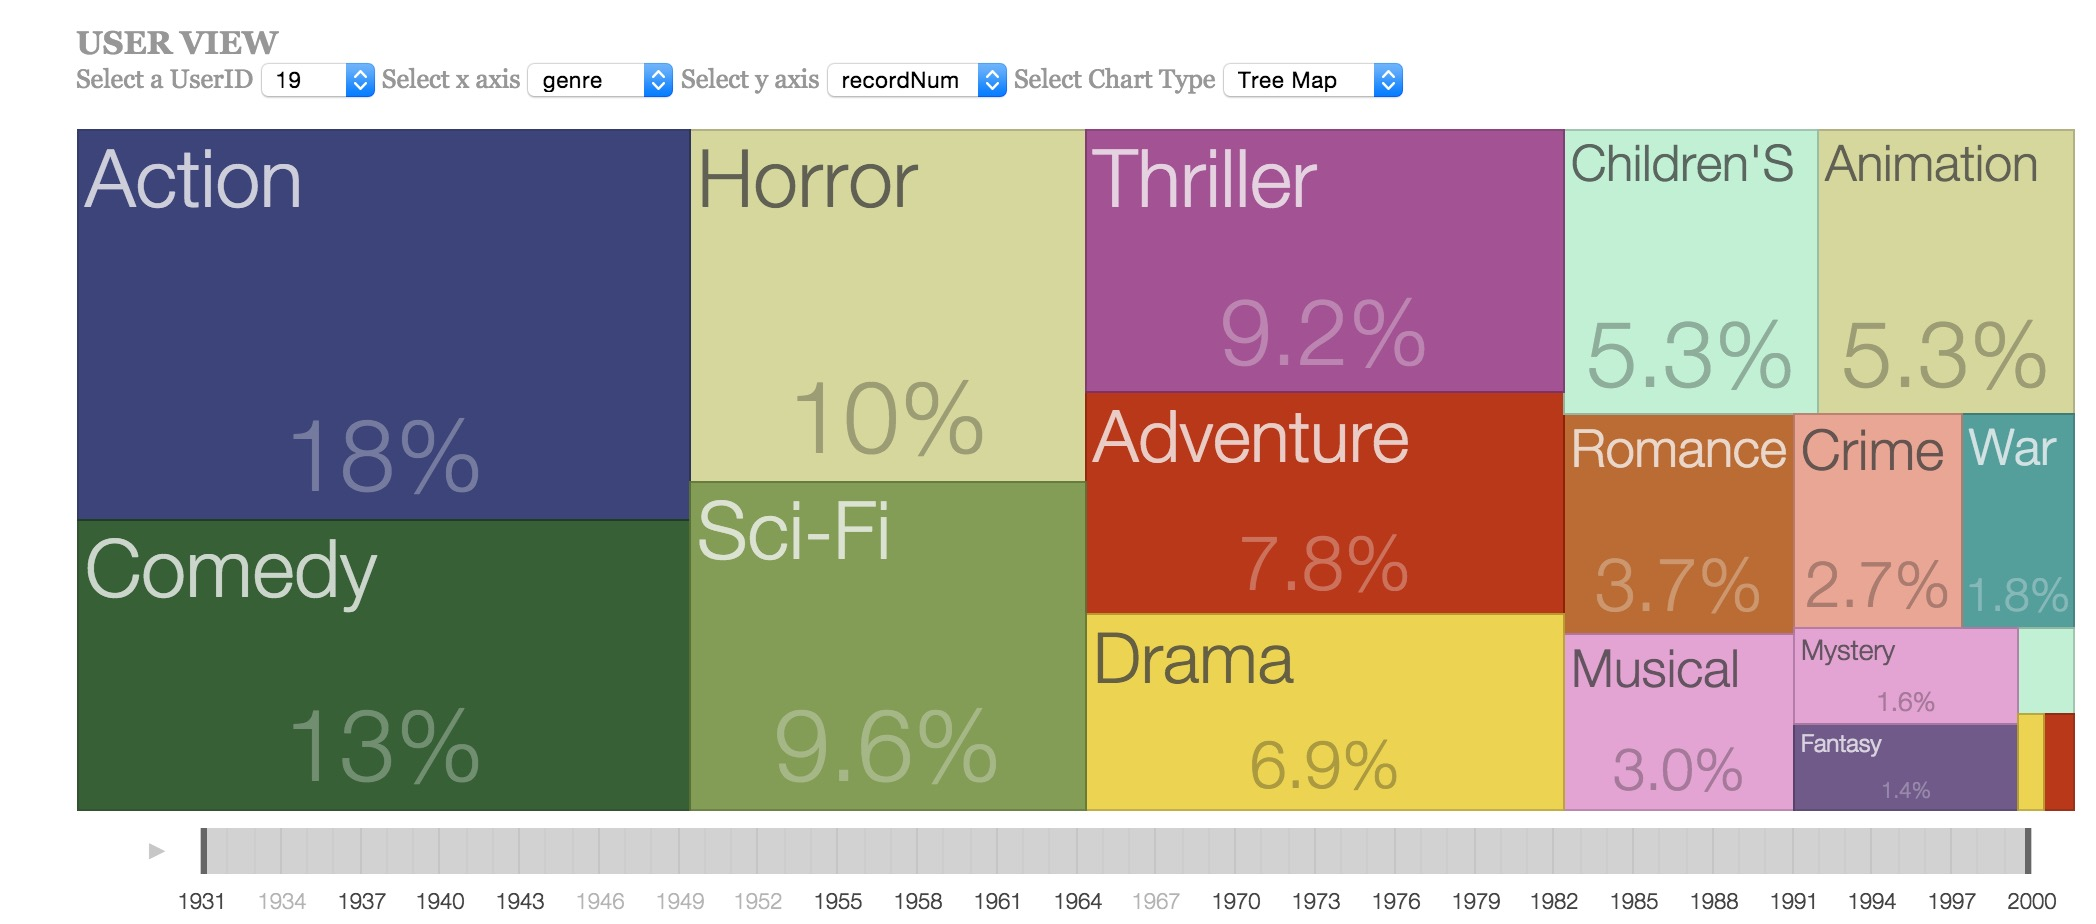
\includegraphics[width=.7\linewidth]{fin_7.png}
}
\caption{Dependencies of users and movies}
\label{fig:fin_7}
\end{figure}

\begin{figure}[h]
\centering{
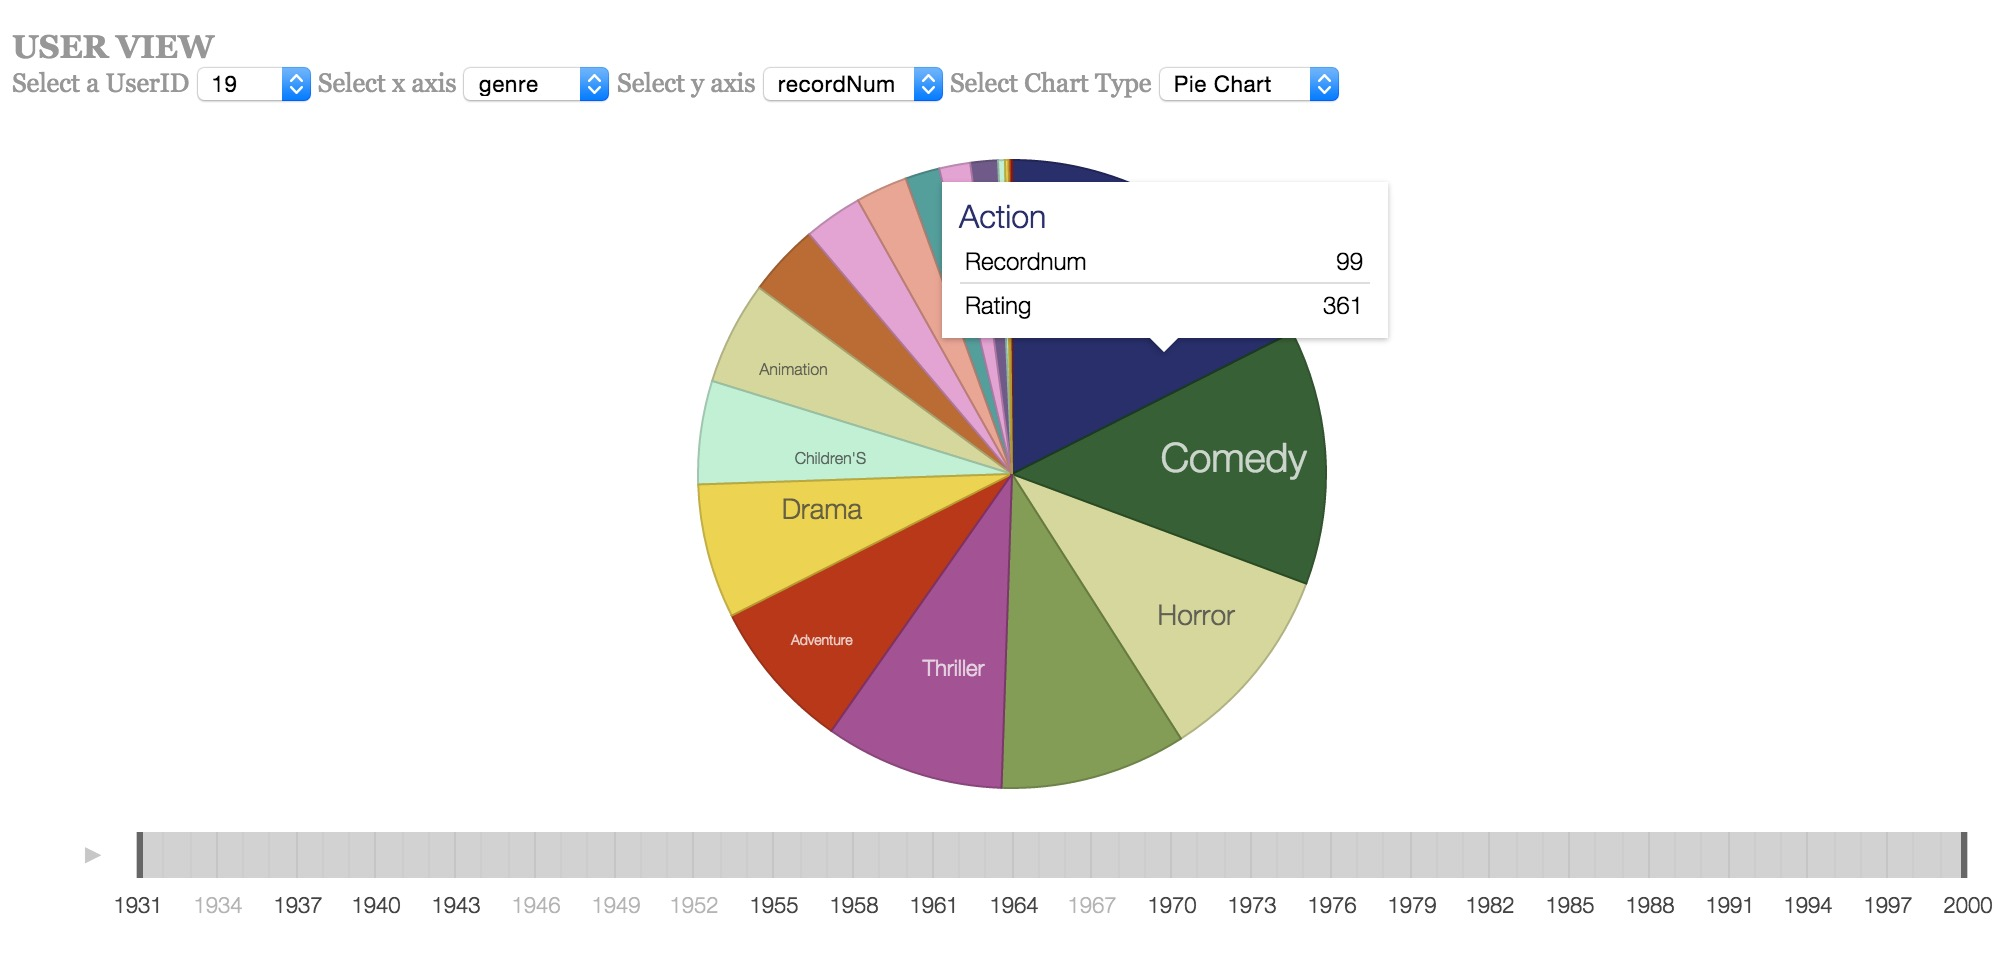
\includegraphics[width=.7\linewidth]{fin_8.png}
}
\caption{Dependencies of users and movies}
\label{fig:fin_8}
\end{figure}


\subsubsection{Geography Map}

We have also implemented a geo map in movie view. For movieID 1, we can see that CA has most user ratings. And ND has the highest average, but the recordNum is only 4. For details, please see Figure \ref{fig:fin_9} and Figure \ref{fig:fin_10}.

\begin{figure}[h]
\centering{
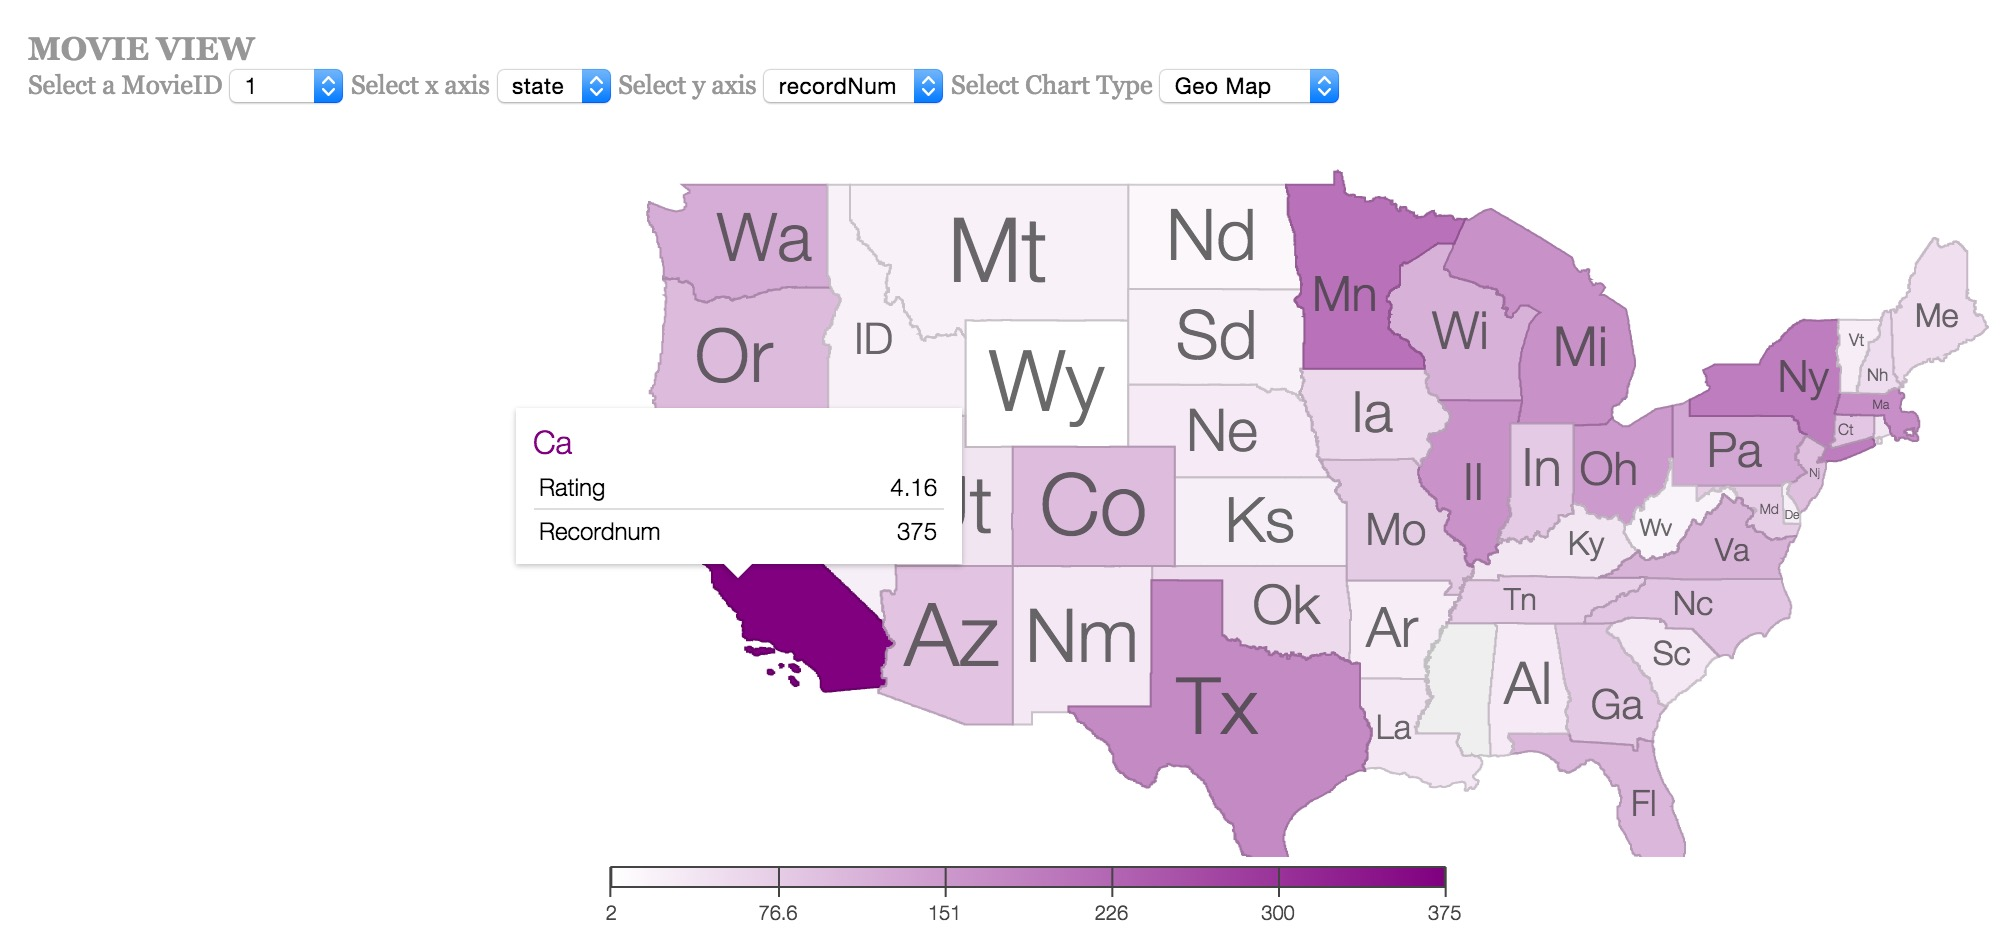
\includegraphics[width=.7\linewidth]{fin_9.png}
}
\caption{Dependencies of users and movies}
\label{fig:fin_9}
\end{figure}

\begin{figure}[h]
\centering{
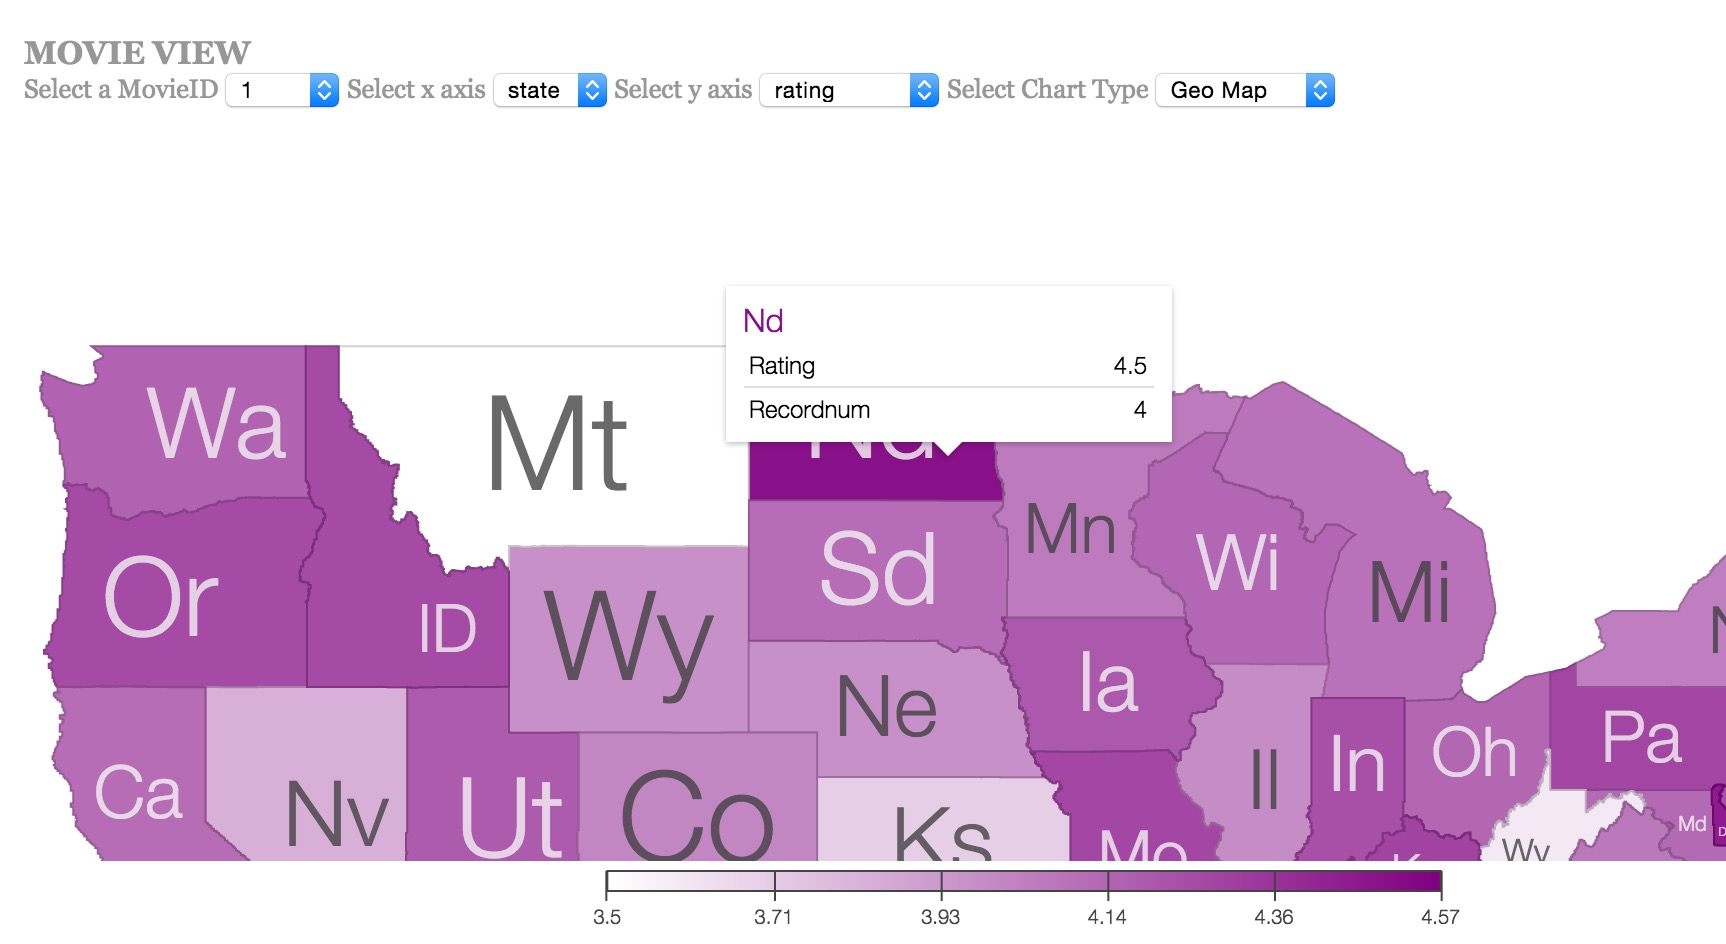
\includegraphics[width=.7\linewidth]{fin_10.png}
}
\caption{Dependencies of users and movies}
\label{fig:fin_10}
\end{figure}

\subsubsection{Other Interesting Features}

1. We have implemented a widget to show the evolution over time. If you click the small button on the left of the timeline, the range will move one step forward every second.


2. If you click an element in the chart of user view, and the element is corresponding to only one movie, then the movie view will also update based on that selected movie.

\section{Evaluation}

What do we learn about the data by using our visualizations?

We find some interesting patterns inside our dataset.
\begin{itemize}
\item Males usually give higher ratings for action movies, crime movies and thrillers than females, while females usually give higher ratings for children��s movies, animations and comedies.
\item The number of ratings for one genre of movies has no relation with the corresponding average rating. Although comedies, dramas and action movies do not have higher average ratings, they gain much more ratings from all kinds of people. Few people give ratings for documentaries and film noirs. However, these two kinds of movies gain the top two average ratings. It seems that only a few people pay attention to them and give them high ratings. For the majority of people, they even do not realize the existence of these movies.
\item Old movies usually gain higher ratings than new movies. The reason may be that old movies rated by people are usually classic movies. It is not surprising for these classic movies to gain high ratings.
\item People in different locations (i.e. states) like to see different kinds of movies. For example, people in Utah give higher ratings for mystery movies than people in other states. However, people in Utah give lower ratings for romance movies and horror movies than people in other states.
\end{itemize}

How do we answer our questions?

\begin{itemize}
\item The first question is how to tell people which movie they may like to see. In our visualization, users can use filters and choose people's attributes that they have and see the output.

\item The second question is for people in different ages how to check what their favorite movies are and the average rating of each
certain movie. Based on our visualization, we can provide the services for users to search the information they want to check about the movies. The information can be related with different ages.

\item The third question is how to help the movie makers to investigate who like their movies best. Our visualization will also benefit the movie makers and help them to make movies that more people like to watch. Since we have done some data analysis and generated a lot of aggregation information, movie makers can easily check the information and find what they need. For example, they can find how age information, location information and gender information have an influence on people's ratings.
\end{itemize}

How well does our visualization work, and how could we further improve it?

\begin{itemize}
\item In our opinion, our visualization can really satisfy user needs. We use all kinds of charts to represent static visualization models. We use filters to represent interactive visualization models. We also use a map to represent geo-location information.
\item We can combine the current data analysis with recommending new movies for users. By using the rating data, we can perform the collaborative filtering algorithm and recommend interesting movies for users. If there is more time left for us, we can represent the recommendation information in our visualization design.
\item We can also try connecting our JavaScript code to MySQL server. Of course, the major issue that we should deal with is how to design the structure of each table, build the indices and use the cache strategy.
\item We can further beautify our visualization, such as adding some background images and using some novel JavaScript libraries.
\end{itemize}

\pagebreak
\restoregeometry
\begin{thebibliography}{}
\bibitem{WWW2001}
B. Sarwar, G. Karypis, J. Konstan, and J. Riedl. Item-based collaborative filtering recommendation algorithms. In \textit{WWW}, pages 285-295, 2001.

\bibitem{IEEE2003}
G. Linden, B. Smith, and J. York. Amazon. com recommendations: Item-to-item collaborative filtering. In \textit{Internet Computing, IEEE}, 7(1), pages 76-80, 2003.

\bibitem{IJCAI2013}
D. Jannach. Tutorial: Recommender systems. In \textit{IJCAI}, 2013.

\bibitem{AAAI1998}
C. Basu, H. Hirsh, and W. Cohen. Recommendation as classification: Using social and content-based information in recommendation. In \textit{AAAI/IAAI}, pages 714-720, 1998.

\bibitem{DL2000}
R. Mooney and L. Roy. Content-based book recommending using learning for text categorization. In \textit{Proceedings of the fifth ACM conference on Digital libraries}, pages 195-204, 2000.

\bibitem{ELIS2000}
R. Burke. Knowledge-based recommender systems. In \textit{Encyclopedia of library and information systems} 69, Supplement 32, pages 175-186, 2000.

\bibitem{WWW2008}
B. Sigurbj{\"o}rnsson and R. V. Zwol. Flickr tag recommendation based on collective knowledge. In \textit{WWW}, pages 327-336, 2008.

\bibitem{WWW20082}
S. Debnath, N. Ganguly, and P. Mitra. Feature weighting in content based recommendation system using social network analysis. In \textit{WWW}, pages 1041-1042, 2008.

\bibitem{UCS2011}
M. Pham, Y. Cao, and R. Klamma. A clustering approach for collaborative filtering recommendation using social network analysis. In \textit{J. UCS}, 17(4), pages 583-604, 2011.

\bibitem{RS2009}
O. Phelan, K. McCarthy, and B. Smyth. Using twitter to recommend real-time topical news. In \textit{Recommender systems}, pages 385-388, 2009.

\bibitem{IR2011}
O. Phelan, K. McCarthy, M. Bennett, and B. Smyth. Terms of a feather: Content-based news recommendation and discovery using twitter. In \textit{Advances in Information Retrieval}, pages 448-459, Springer Berlin Heidelberg, 2011.
\end{thebibliography}
\end{document}
